\documentclass[longabstract, english, mgr]{iithesis}
\usepackage[utf8]{inputenc}
\usepackage{enumitem}
\usepackage{filecontents}
\usepackage{url}
\usepackage{breakcites}
\usepackage{graphicx}
\usepackage{caption}
\usepackage{subcaption}
\usepackage{tabularx}
\usepackage[T1]{fontenc}
\usepackage{titlesec}
\usepackage{amsthm}
\usepackage{amsmath}
\usepackage{amsfonts}
\usepackage{bbm}
\usepackage{float}
\usepackage{afterpage}
\usepackage{makecell}
\usepackage{multirow, fixltx2e}

\graphicspath{{./images/}}

\titleformat{\chapter}[block]{\normalfont\huge\bfseries}{\thechapter.}{5pt}{\huge}
\titlespacing*{\chapter}{0pt}{-19pt}{25pt}
\titleformat{\section}[block]{\normalfont\Large\bfseries}{\thesection.}{5pt}{\Large}
\titleformat{\subsection}[block]{\normalfont\large\bfseries}{\thesubsection.}{4pt}{\large}

\newcommand\blankpage{\null\thispagestyle{empty}\newpage}
\newcommand\numberedchapter[1]{\setlength\topskip{3cm}\chapter{#1}\setlength\topskip{0cm}}

\newtheoremstyle{default_theorem_style}
  {1em plus .2em minus .1em}%   Space above
  {1em plus .2em minus .1em}%   Space below
  {\slshape}%  Body font
  {}%          Indent amount (empty = no indent, \parindent = para indent)
  {\bfseries}% Thm head font
  {.}%         Punctuation after thm head
  {0.5em}%     Space after thm head: " " = normal interword space;
     %         \newline = linebreak
  {}%          Thm head spec (can be left empty, meaning `normal')


\theoremstyle{default_theorem_style}\newtheorem{theorem}{Theorem}
\theoremstyle{default_theorem_style}\newtheorem{definition}{Definition}

\polishtitle    {Uzupełnianie grafów wiedzy przy użyciu transformerów}
\englishtitle   {Transformer-based knowledge graph completion}
\author         {Dawid Wegner}
\advisor        {dr hab. Jan Chorowski}
\date           {29 września 2021}

\englishabstract{Knowledge graphs play a crucial role in many systems used by billions of people, providing access to
relations between various objects present in our daily life. \ In parallel, the knowledge contained in them is often
incomplete.\ Therefore, the problem of completing knowledge graphs is becoming more and more important for
humanity.\ The fact that most of them are very dynamic systems, makes it impossible for humans to fill out
missing relations by hand.\ In the past, simple heuristic approaches have been tried to tackle the stated problem,
but they covered only simple cases like inverse relations.\ With the rise of machine learning techniques, researchers
started developing various model-based approaches, making tremendous progress over the past few years.\newline

\noindent At this time, the most successful methods are based on convolutional neural networks, reinforcement learning
and graph neural networks.\ In this thesis, we tackle the stated problem with transformer-based models, which have
already found their applications in many sequence-to-sequence problems, outclassing other approaches.\ In particular,
we develop a model operating on single edges as well as explore several approaches that add graph-based context to the
model.\ Additionally, we compare the developed methods with other successful approaches on two popular benchmark
datasets, called FB15K-237 and WN18RR.
}

\polishabstract {Grafy wiedzy odgrywają kluczową rolę w wielu systemach używanych przez miliardy ludzi, zapewniając
dostęp do relacji między przeróżnymi obiektami obecnymi w naszym codziennym życiu.\ Jednocześnie, wiedza w nich zawarta
jest często niepełna.\ Wynika stąd, że problem uzupełniania grafów wiedzy staje się coraz ważniejszy dla
ludzkości.\ Fakt, że większość z nich to układy bardzo dynamiczne, uniemożliwia ludziom ręczne uzupełnianie brakujących
relacji.\ W przeszłości próbowano prostych podejść heurystycznych do rozwiązania przedstawionego problemu, ale działały
one tylko w prostych przypadkach, takich jak odwrotne relacje.\ Wraz z rozwojem technik uczenia maszynowego naukowcy
zaczęli opracowywać różne podejścia oparte na modelach, osiągając ogromne postępy przez ostatnie kilka lat.\ Obecnie
najlepsze metody opierają się na splotowych sieciach neuronowych, uczeniu ze wzmacnianiem i grafowych
sieciach neuronowych.\newline

\noindent W tej pracy podejmujemy postawiony problem przy pomocy modeli opartych na transformerach, które zdążyły już
znaleźć swoje zastosowanie w wielu problemach mapowania sekwencji wejściowej do sekwencji wyjściowej, jednocześnie
deklasując inne podejścia.\ W szczególności opracowujemy model operujący na pojedynczych krawędziach, a także badamy
kilka podejść, które dodają do modelu kontekst oparty na grafie.\ Dodatkowo, porównujemy opracowane metody z innymi
udanymi podejściami na dwóch popularnych zestawach danych, nazwanych FB15K-237 i WN18RR.
}

\begin{document}

\numberedchapter{Introduction}

In the following introductory chapter, we will define the notion of knowledge graph along with the problem of
completing it.\ Furthermore, we will discuss the main motivations for solving the considered problem and give an
overview of the past work.\ Finally, we will provide an outline of our approach to the problem of completing a
knowledge graph.

\section{Problem formulation}

Consider a set of objects $e \in E$ and a set of relations $r \in R$.\ Formally, a \textbf{knowledge graph} is a set
of triples $(e_1, r, e_2) \in K$, which represents relations between the considered objects.\ Particularly,
$e_1 \in E$ is called to be in a (directed) relation $r \in R$ with $e_2 \in E$ if and only if
$(e_1, r, e_2) \in K$.\ We will refer to an object $e \in E$ as an \textbf{entity} and to an object
$r \in R$ as a \textbf{relation}.\ Besides it, when considering a triple $(e_1, r, e_2)$, we will refer to
$e_1, e_2$ as a \textbf{head entity} and a \textbf{tail entity}, respectively.\ From the practical perspective, we
can think of our structure as a directed graph where vertices are represented by entities and edges are labelled
by relations.\ A toy example illustrating a knowledge graph is shown in
\textit{Figure} \ref{fig:knowledge_graph}.\newline

\noindent While we would expect a knowledge graph to contain any information that is useful for a user, in practise
the vast majority of relations are missing.\ This fact becomes intuitive when one realizes that adding one edge
to a graph can add information about relations between several entities that are not adjacent to the added
edge.\ As a result, the number of missing relations can grow exponentially with the increase of the number of
edges.\ The problem of finding new relations in a knowledge graph is known
as \textbf{Knowledge Graph Completion}.\newline

\noindent Formally, we are given a knowledge graph $G$ and our goal is to find triples $(e_1, r, e_2) \in K$ that
are likely to represent true facts.\ Specifically, given a head entity $e_1 \in E$ and a relation $r \in R$, we
aim to find a tail entity $e_2 \in E$, such that $(e_1, r, e_2)$ is true.\ The analogous goal can be defined for
a missing tail entity, given a head entity and a relation.\ The knowledge graph completion methods can be divided
into those that extract information only from a graph and those that utilize additional information e.g.\ text-based
definitions of entities.\ In this thesis, we only leverage information that is contained in a given graph,
particularly our models falls into the graph-only category.

\begin{figure}[H]
\centering
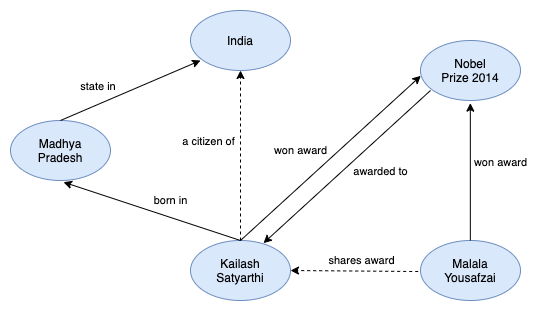
\includegraphics[scale=0.6]{knowledge_graph}
\caption{An example of a knowledge graph. Solid edges represent triples that are present in the knowledge graph, while
dashed edges represent knowledge that is missing, but can be inferred directly from the graph.}
\label{fig:knowledge_graph}
\end{figure}


\section{Motivations for solving the problem}

The first question to ask could be whether we really need a sophisticated model in order to complete a knowledge
graph.\ Actually, most of knowledge graphs are very dynamic systems that evolve over time, making it impossible for
humans to complete them by hand.\ Additionally, the problem of completing a knowledge graph is the very complex
one.\ While simple heuristic approaches have been tried in the past, they only covered simple cases like inverse
relations.\ As a result, in order to extract more sophisticated relations, we need a model that understands
entities and their relations more deeply.\newline

\noindent Solving the stated problem is motivated further by the fact that it has many real-world
applications.\ First of all, consider a situation when you ask a voice assistant to answer a question about the
nationality of your favourite actor.\ The answer to this question can be fetched from a knowledge graph, assuming that
it is complete enough to contain this information.\ In order to be able to answer more questions, one needs to assure
that the graph is complete.\ The class-leading voice assistants and search engines actually make use
of knowledge graphs to provide answers to users' questions.\ Those graphs are developed by parsing online
encyclopedias like Wikipedia as well as news websites and as a result are often incomplete.\newline

\noindent Knowledge graphs are are also useful in many other areas.\ For instance, they are used to boost
recommendation engines of popular content and social media platforms.\ Furthermore, knowledge graphs are leveraged
in the healthcare industry, enabling medical researchers to gain more insights from data.\ Additionally, they are
also used to represent the relations between words in human languages.\ Lastly, knowledge graphs are leveraged by
financial services to secure human decisions and prevent money laundering initiatives.


\section{Related work}

In the recent years, various approaches have been tried to tackle the problem of knowledge graph completion.\ The most
successful ones are based on data-driven models, often called machine learning models.\ These methods will be
discussed more deeply in the \textit{Chapter} \ref{chapter:background}.\ For our task specifically, we can divide the
considered models into ones that operate on triples alone (representing graph edges) i.e.\ context-free methods and
those that utilize graph context e.g.\ neighbours of a head/tail entity.\ Recently, a new branch of models that
leverage additional text-based information has been established, but those models are not considered in this
thesis.\newline

\noindent While the first context-free methods were proposed in 2013, the new models are still developed, surpassing
the old ones.\ One of the first baseline models, learning latent representations of entities and relations, is known
as the \textit{TransE} model introduced in \cite{transe_model}.\ The model was later extended in \cite{stranse_model}
to \textit{STranse}, which allows entities to have relation-specific representations.\ Several other
improvements, utilising convolutional neural networks to learn better representations, have been proposed,
including \textit{ConvE} model presented in \cite{conve_model}.\ While many other context-free models have been
developed, they retain the same quality of predictions.\ Therefore, we compare our methods only with the
above-mentioned models.\newline

\noindent In the past few years, several models have been developed to utilise context of a given graph.\ The first
applications of those models to the considered problem have been proposed back in 2017.\ While many of the
approaches failed to surpass context-free models, a few models have provided a considerable quality
improvement.\ One of the successful approaches include \cite{go_for_a_walk_model} that tries to walk through a graph
to find a matching entity.\ The other popular methods are based on graph neural
networks, especially on the \textit{GCN} architecture proposed in \cite{gcn_model}.\ The best-performing ones
include the \textit{SACN} model presented in \cite{sacn_model} and recently developed \textit{CompGCN} model
introduced in \cite{comp_gcn_model}.\ Although many other models have been proposed, as shown in
\cite{re_evaluation}, some of researchers have reported inflated quality results due to improper evaluation
protocol.\ Therefore, we compare our models only with the models discussed above.

\section{Our approach}

One of the most ground-breaking machine learning architectures in the recent few years is the \textit{Transformer} model
introduced in \cite{transformer_model}.\ It has been successfully applied to many sequence-to-sequence problems,
outclassing other models.\ Moreover, several improvements have been proposed to the original architecture.\ For
instance, the authors of \textit{BERT}, introduced in \cite{bert_model}, proposed a language
representation model that is pretrained on specially designed tasks to later boost its quality on the downstream
task.\ Just like in the case of the original transformer architecture, the proposed BERT model outperformed other
architectures in many classification tasks, especially in the area of Natural Language Processing.\ Following the
success of the proposed approach, researchers have developed even better architectures.\ One of the recently
developed models include \textit{ALBERT}, proposed in \cite{albert_model}, that is a lite version of the BERT model.
The other interesting approach is taken in \cite{electra_model}, which trains the BERT model adversarially.\ Besides it,
several components of the baseline architecture have been improved over time, for instance the authors of
\cite{layer_normalization_in_transformers} showed that changing the location of normalization layers lead to better
performance of the model.\newline

\noindent Motivated by the recent advancements in the transformer-based models, we decided to tackle to the problem
of knowledge graph completion, using the above-mentioned models.\ In particular, we explore both
context-free and contextualised methods, determining whether a transformer can benefit from an additional context
information.\ Besides it, we compare the developed methods with the related models on two benchmark datasets, known
as WN18RR and FB15K-237.

\numberedchapter{Background}\label{chapter:background}

In this chapter we will review the theory behind the techniques used to complete knowledge
graphs.\ \textit{Section} \ref{sec:neural_networks}
is devoted to the basic properties and concepts of neural networks.\ In the subsequent sections we discuss more
specialized models that are used to tackle the stated problem.\ In
\textit{Section} \ref{sec:graph_embedding_methods} and \textit{Section} \ref{sec:graph_neural_networks} we cover
models learning graph representations.\ \textit{Section} \ref{sec:reinforcement_learning} provides an overview of
how reinforcement learning can be utilized to complete knowledge graphs.\ In \textit{Section}
\ref{sec:transformers} we discuss the transformer architecture, which is the main building block for our
methods.\ Finally, in \textit{Section} \ref{sec:background_models} we show how the methods discussed in the previous
sections have been utilized in the past to solve the considered problem.

\section{Artificial neural networks}\label{sec:neural_networks}

Neural networks are machine learning models inspired by a human brain.\ While the first neural models have
been proposed decades ago, their popularity was very limited due to the poor performance.\ In the recent
few years, the situation has changed as researchers developed sophisticated algorithms to optimize such models while
in parallel computing resources have been grown significantly.\ At this point, neural networks have dominated other
approaches to artificial intelligence, finding applications in practically every area of human life.

\subsection{Feed-forward neural networks}\label{subsec:feed_forward}

\noindent Formally, a neural network is a complex mathematical function that maps input vectors to output
vectors.\ One of the simplest neural network can be defined using the formula
\begin{equation}\label{eq:one_layer_network}
y = f(W x + b)\ ,
\end{equation}
where $x, y$ denotes input and output vectors of size $n$, $m$ respectively, $W$ is a $n \times m$ matrix of
parameters, $b$ denotes a so-called bias vector of size $m$ and $f$ is a fixed activation function that
adds non-linearity to our formula.\ The more complex neural network would repeat the process of mapping vectors several
times e.g.
\begin{equation}\label{eq:multi_layer_network}
y = f_3(f_2(f_1(W_1 x + b_1) W_2 + b_2) W_3 + b_3)\ .
\end{equation}
Due to its linear form, such network is often called a feed-forward neural network.\ An input vector $x$ is often
called an input layer, the intermediate vectors are called hidden layers and an output vector $y$ is called
an output later.\ The above-defined neural network has 2 hidden layers, defined as outputs of $f_2$ and $f_3$
activation functions.\ A feed-forward neural network can be illustrated in the form presented in
\textit{Figure} \ref{fig:neural_network}.\newline

\noindent While we have shown how a neural network maps input vectors to output vectors, it is still unclear how such
model can be leveraged to make predictions.\ The idea is to utilise so-called training dataset that is composed of
input, expected output pairs.\ It is used to learn our neural network how to map inputs to
outputs.\ In order to make use of the training dataset, one needs to convert given inputs and outputs
to real-valued vectors.\ As neural networks are supervised on training data, they belong to the subcategory of machine
learning called supervised learning.\ After training a neural network, its quality is rated on a validation dataset,
which is disjoint with training dataset, providing an estimation of quality for examples that were not seen by the
model.\ In particular, neural networks are known for fitting to training data too tightly while providing a poor
quality on unseen examples.\ The techniques for preventing this phenomena, called overfitting, are discussed in
\textit{Subsection} \ref{subsec:overfitting}.\ In case multiple models are tested, the validation set is used to pick
the best one, while the quality of the chosen model is additionally evaluated on a test dataset as it can be a little
biased to the validation dataset.\ The task-specific functions that rate models are often called
evaluation metrics.\newline

\begin{figure}[t]
\centering
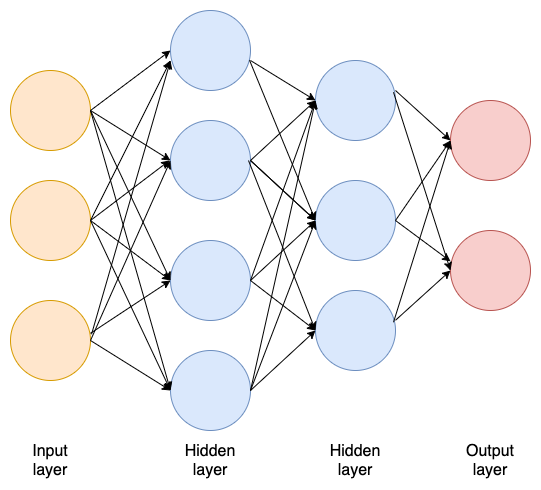
\includegraphics[scale=0.45]{neural_network}
\caption{An example of a feed-forward network containing 2 hidden layers (marked in blue). The input layer
(marked in orange) is composed of three neurons, while the output layer (marked in red) is composed of two neurons.}
\label{fig:neural_network}
\end{figure}

\noindent In order to fit a neural network to a given training dataset, one needs to find parameters that provide the
best correspondence between predicted output vectors and expected output vectors.\ The trainable parameters include
linear transformation matrices and bias vectors.\ For instance, for a neural network defined by
\textit{Equation} \ref{eq:multi_layer_network}, the trainable parameters include
$W_1, W_2, W_3, b_1, b_2, b_3$.\ Intuitively, the more parameters the network has, the higher its expressiveness.\ The
optimization process of neural networks is performed by a specially designed algorithm that is
described in \textit{Subsection} \ref{subsec:optimization}.

\subsection{Convolutional neural networks}

Consider a task of classifying images into one of given categories e.g.\ $C = \{cat, dog\}$.\ It is easy to develop
a feed-forward neural network that would treat images as input vectors and apply a few layers in order to obtain
1-dimensional output, representing a probability of an image to represent a cat.\ Actually, this approach works
decently, but it suffers from the overfitting problem, causing that the quality of such model on unseen examples is
lower than expected.\ The problem with the feed-forward approach is that such network tries to learn the dependencies
between all pixels at the same time.\ The more natural way would be to train a model to firstly learn some
low-level patterns like edges and then to recognize larger objects.\ Convolutional networks are models that implement
this idea, enforcing the model to learn from neighbouring features.\newline

\noindent In the case of convolutional networks, an input vector is represented by a 3-dimensional tensor of size
$H \times W \times C$ interpreted as a height, width and  the number of channels respectively.\ A single convolutional
layer maps the input tensor, often called an input feature map, to the output tensor, which is called an output
feature map.\ A single output neuron is computed by multiplying (element-wise) a patch of input feature map with
a learnable 3D matrix of size $\tilde{h} \times \tilde{w} \times C$.\ The process is repeated by going through the
input feature map with a sliding window of size $\tilde{h} \times \tilde{w} \times C$.\ The whole process for an input
feature map with the number of channels $C = 1$ is shown in \textit{Figure}
\ref{fig:convolutional_network}.\ The above-defined algorithm maps an input feature map of size
$H \times W \times C$ to an output feature map of size $\tilde{H} \times \tilde{W} \times 1$, using a learnable
kernel matrix of size $\tilde{h} \times \tilde{w} \times C$.\ In practice, this process is repeated $\tilde{C}$ times
for independent kernel matrices, where $\tilde{C}$ is called the number of filters.\ In this case, the output feature
map is of size $\tilde{H} \times \tilde{W} \times \tilde{C}$.\newline

\noindent Convolutional networks are learnt by modifying parameters contained in kernel matrices.\ Mathematically,
nothing prevents composing a neural network that contains a few convolutional layers followed by feed-forward
layers.\ In the first case inputs can be treated as 3D tensors, while in the latter case, they can be transformed
to 1D representations.

\begin{figure}[t]
\centering
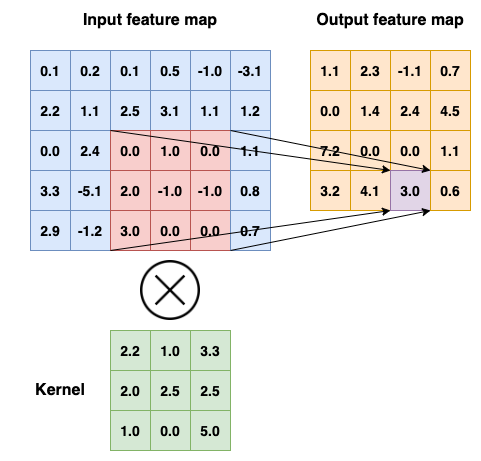
\includegraphics[scale=0.48]{convolutional_network}
\caption{An example of how convolutional layer maps input feature map (marked in blue) to output feature
map (marked in orange).\ A single patch (marked in red) is multiplied element-wise with a learnable kernel matrix
(marked in green) in order to produce one output feature (marked in purple).\ A sliding window goes though the entire
image, multiplying input patches with a kernel matrix.\ Note that while in this example an input feature map contains
only one channel, in the more general case of $C$ channels, the kernel matrix would be of size $C \times 3 \times 3$.}
\label{fig:convolutional_network}
\end{figure}

\subsection{Loss functions}\label{subsec:loss_functions}

In order to train a model, one needs to define a similarity between predicted outputs $\tilde{y}$ and ground-truth
outputs $y$.\ A function that defines this similarity is called a loss function and depends on a considered
task.\ One popular case is when a target variable $y$ is continuous and the loss function should be based on the
distance between $y$ and $\tilde{y}$.\ In the field of machine learning, this is often called a regression
task.\ While many different functions can be designed to optimize such model, the most popular one is
$$
L_2(y, \tilde{y}) = ||y - \tilde{y}||_2 = \sum_i (y_i - \tilde{y}_i)^2\ ,
$$
which is called L2 loss function.\ The other case is when $\tilde{y}$ represents an unnormalised probability
distribution for a set of established classes (e.g.\ $C = \{cat, dog, rabbit\}$), while $y$ is so-called one-hot
vector encoding classes that are true for a specific sample as $1.0$ and classes that are false as $0.0$.\ In
this case, the popular choice is to first apply a softmax function to normalize $\tilde{y}$
$$
\hat{y}_i = \frac{e^{\tilde{y}_i}}{\sum_j e^{\tilde{y}_j}}
$$
and then apply cross-entropy loss function
$$
L(y, \hat{y}) = -\sum_i y_i log(\hat{y}_i)\ ,
$$
penalizing predictions for classes for which $y_i > 0$.\ Except natural intuitions that the above-defined loss
function should be minimized in order to provide a good estimate of $y$, it has also mathematical foundations that
can be found in \cite{goodfellow_book}.\ In case there are only two classes, the discussed loss function is often
called binary cross entropy, while the task of optimising such function is referred as binary classification.

\subsection{Optimization}\label{subsec:optimization}

In the previous subsections we mentioned that a neural network is optimized by adjusting parameters contained in
matrices and bias vectors.\ Besides it, we defined a loss function that should be minimised in order to fit to the
expected outputs.\ In this subsection, we show how to actually minimize a loss function.\newline

\noindent First of all, our training data samples should be split into batches of fixed size $B$, which is often
referred as batch size.\ In each training step, a batch of inputs is pushed to a model, and its parameters
are slightly modified to lower the value of a loss function.\ In order to minimize it, a technique called gradient
descent is utilised.\ Specifically, it computes a gradient of the loss function with respect to all parameters,
using so-called backpropagation algorithm.\ As a result, the method obtains a vector that defines the direction that
should be followed to lower the value of the loss function.\ Then, the vector of parameters is updated by applying
$$
\theta_{k + 1} = \theta_k - \alpha \nabla_{\theta} L(\tilde{Y}, Y)\ ,
$$
where $\alpha$ is called a learning rate.\ The process of updating parameters is performed for all training batches and
repeated $E$ times, where $E$ is referred as the number of epochs.\ While this naive algorithm can stuck in a
local minima, several advancements have been developed in order to make it possible to converge to a global minima.\ One
of the currently popular approach is known as Adam optimizer, introduced in \cite{adam_optimizer}.\ Over time,
researchers have also developed specialized layers that increase the convergence rate.\ One of the most successful
layers is Batch Normalization, proposed in \cite{batch_normalization}, normalizing batches of inputs to the
parameterised Gaussian distribution.\ The other popular alternative is Layer Normalization, introduced
in \cite{layer_normalization}, which normalizes each sample separately, making the computations more precise for
small batch sizes.

\subsection{Preventing overfitting}\label{subsec:overfitting}

Neural networks are great in recognising patterns in training data.\ In particular, a feed-forward neural network with
1 hidden layer can represent any function.\ But in practice, we are not interested in a model that remembers all
training data samples i.e.\ overfits to them.\ Instead, we would like to design models that generalize well, providing
good quality of predictions on unseen examples.\newline

\noindent One popular way of enforcing the network to generalize is adding a dropout layer \cite{dropout}.\ The
idea is to (in each training step) set some random subset of neurons after a specific layer
to $0.0$ and rescale the other neurons by $1.0\ /\ (1.0 - r)$, where $r$ (often called a dropout rate) denotes
the percentage of neurons that are set to $0.0$.\ The neurons that are set to $0.0$ can be treated as removed.\ The
intuitive explanation of how dropout is applied during the training process, is shown in
\textit{Figure} \ref{fig:dropout}.\ During the evaluation of the network on unseen examples, all neurons are included
and no rescaling is applied.\ The intuition behind this approach is that it enforces the network to spread out its
weights to many neurons rather than relying on a small number of connections.\newline

\noindent The other technique to reduce the overfitting is to add an additional loss that penalizes model's
parameters.\ The common way of applying this idea is to add a regularization term to the loss function
$$
L(y, \tilde{y})^{\theta} = L_m^{\theta}(y, \tilde{y}) + \lambda \sum_i \theta_i^2\ ,
$$
where $\theta$ denotes a vector of parameters, $L_m$ is the loss given by the model and $\lambda$ is a parameter
controlling the regularization strength.\ The above-defined technique is often called a weight decay.\ The intuition
behind this approach is that it enforces the network to keep parameter values close to $0.0$ and to avoid extreme
values, making it less flexible.\newline

\begin{figure}[t]
\centering
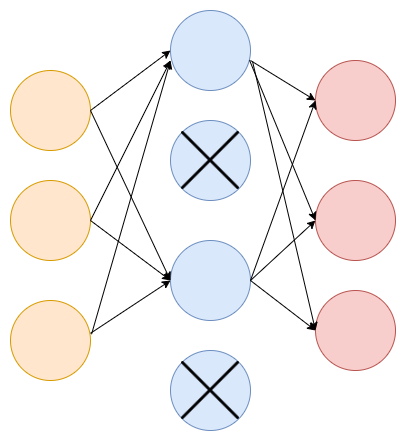
\includegraphics[scale=0.42]{dropout}
\caption{An illustration of dropout to applied to a hidden layer (marked in blue). The crossed out neurons are set
to $0.0$, which has an effect of ignoring their input and output connections.\ In this case dropout rate $r = 0.5$.}
\label{fig:dropout}
\end{figure}

\noindent The other regularization technique, which is designed for classification tasks, is label
smoothing.\ The idea behind this method is to replace hard $c \in \{0, 1\}$ labels with their soft
versions.\ Specifically, when label smoothing parameter is set to $s \in (0, 1)$, true labels are replaced with
$(1 - s) + s\ /\ N$, while false labels are replaced with $s\ /\ N$, where $N$ denotes the total number of
classes.\ The main motivation behind this approach is that the training dataset can contain mistakenly labeled
examples.\ Another common situation is when multiple output labels are correct, while a dataset is constructed in a way
that only one label is true for a specific sample.\ In this case, label smoothing encourages a model to assign some
non-zero probability to each class.\ In particular, it can assign higher probabilities to labels that may be correct.

\section{Graph embedding methods}\label{sec:graph_embedding_methods}

Consider a dataset containing users' features and the problem of classifying each user to one the specified
categories.\ In order to tackle this task, one may utilise neural networks discussed in
\textit{Section} \ref{sec:neural_networks} to learn a mapping from user's features to categories.\ Now, let's assume
that one of our features is a list of friends of a user.\ In other words, users are interconnected, forming a
graph.\ While we could try to naively encode this information by creating a one-hot vector indicating a list of
friends for each user, there are more sophisticated ways to include this information.\ One of the most successful
approaches is to use graph embedding methods that aim to learn low-dimensional vector representations of nodes.

\subsection{Classification of graph embedding methods}

\noindent Most of embedding methods are unsupervised.\ The goal is to produce generic, continuous representations of
nodes based  on their connectivity.\ The representation of a node is often referred as embedding.\ The learnt
embeddings can be later used by some supervised model to perform a node classification task
(e.g.\ classify users of a social network), link prediction task (e.g.\ predict new friendships) or graph
classification task (e.g.\ classifying chemical structures).\ Most of embedding methods are based on so-called
homophily hypothesis, which says that nodes that are highly interconnected and belong to similar network clusters
should have similar embeddings.\ The other category of considered methods is based on structural equivalence
hypothesis, which states that nodes with similar structural roles in a graph should be embedded closely
together.\ Lastly, while most of methods allow to learn only fixed representations for nodes contained in the training
dataset i.e.\ transductive methods, there exist more specialized methods allowing predictions to be made on unseen
nodes i.e.\ inductive methods.

\subsection{DeepWalk algorithm and its extensions}

One of the baseline models that outclassed previous approaches is DeepWalk, introduced in \cite{deepwalk}.\ At each step
of the algorithm, a random node $v \in V$ is chosen.\ Then, a random path $W = \{w_1, w_2, \dots, w_k\}$ is
constructed by starting in the node $v$ and repeatedly going to one of the neighbours of the last node on the
constructed path.\ The generated paths are later used to enforce nodes having similar neighbours to be closely
embedded.\ Specifically, let $v_j \in W$ be a random node from the generated path and its context to be defined as
a set of nodes $K = \{w_{j - c}, w_{j - c + 1}, \dots, w_{j + 1}, w_{j + c}\}$.\ Now, draw one vertex $v_c \in K$
and define $p(v_c | v_j)$ with the formula
\begin{equation}\label{eq:deepwalk}
p(v_c | v_j) = \frac{e^{R_j C_c^T}}{\sum_k e^{R_j C_k^T}}\ ,
\end{equation}
where $R_i$ denotes the i-th row of the learnable embeddings matrix, while $C_i$ is the i-th row of the learnable
context matrix.\ The goal of the above-defined model is to maximize this probability for the generated $v_j, v_c$
nodes.\ As a byproduct of this procedure, we get the embeddings matrix $R$, such that the i-th row represents the
i-th node.\ The intuition behind this approach is it enforces nodes that have many common neighbours to have similar
embeddings as they are often multiplied with the same context vectors.\ A toy example of how the presented algorithm
could embed a small graph in 2-dimensional space is shown in \textit{Figure} \ref{fig:deepwalk}.\newline

\noindent Interestingly, the presented algorithm was invented previously to embed words in a way that the related ones
have similar representations.\ The original method is called the Skip-gram model and was introduced in
\cite{skipgram}.\ Additionally, to speed up the computation time of \textit{Equation} \ref{eq:deepwalk}, the authors
proposed to replace the original softmax function with a hierarchical softmax, keeping nodes in leaves of a binary
tree.\ The other popular method is to use negative sampling, which tries to maximize
$$
p(v_c | v_j) = e^{R_j C_c^T}
$$
for positive pairs, while minimizing the same formula for negative pairs that are created by drawing two random
words.\ The analogous extensions can be applied to the DeepWalk algorithm.\newline

\noindent While the original DeepWalk algorithm traverses the graph using DFS strategy, other strategies could
be utilised.\ The authors of \cite{node2vec} generalized DeepWalk to choose between one of strategies: BFS, DFS,
going back to the previous node.\ The proposed node2vec algorithm interleaves strategies by selecting a random one in
each step of constructing the path.\ A distribution defining the probability of choosing a specific strategy impacts the
learnt representations.\ Most commonly, the parameters defining a distribution of strategies are finetuned to provide
the best quality.\newline

\begin{figure}[t]
\centering
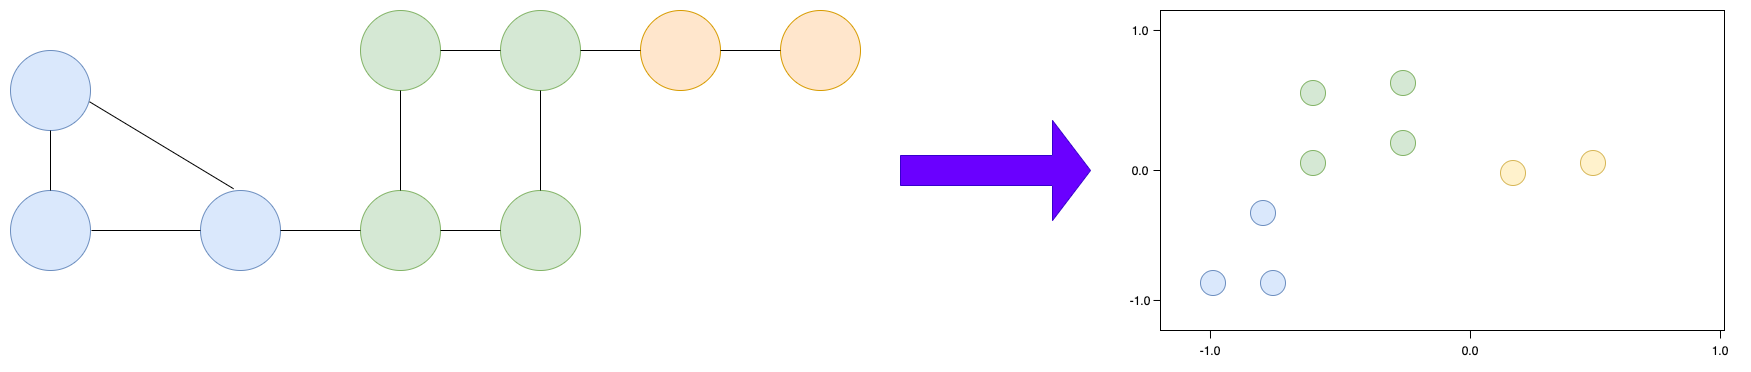
\includegraphics[scale=0.23]{deepwalk}
\caption{An example of how DeepWalk algorithm could embed nodes of a given graph in 2 dimensional space. The nodes
are marked with colors to show the correspondence between the locations in the graph and locations in the embedding
space.}
\label{fig:deepwalk}
\end{figure}

\noindent The other interesting extension proposed in \cite{struc2vec} utilises the DeepWalk algorithm to embed
nodes that have similar structural roles closely together.\ The idea behind struc2vec is to first construct a
graph encoding structural similarities between nodes and then learn embeddings by performing random walks.\ The authors
proposed to define a structural distance between nodes $u, v \in V$ based on the number of neighbours
$R_k(u), R_k(v)$ at specified distances $k \in \{1, \dots, K\}$.\ Then, the constructed distances matrix is utilized
to define the probability of transitioning from $u$ to $v$.\ As a result, random walks enforce nodes of the same
structure to have similar embeddings.

\subsection{Learning representations of unseen nodes}

Though we have shown many extensions of the DeepWalk algorithm, none of them scale to unseen nodes.\ The naive approach
to extend it would be to rerun random walks when new nodes arrive, but it makes the computations very costly.\ In
case the nodes are represented by additional pre-defined features, one may try to learn embeddings by mapping input
features.\ One way of applying this idea is to use a model introduced in \cite{planetoid}.\ The authors propose to
learn a specific supervised task along with the embeddings of nodes at the same time.\ Specifically, one of hidden
layers of the supervised model can be treated as an embedding layer, representing an input node with a given
features.\ In order to enforce the neighbouring nodes to have similar embeddings, random walks are applied to
the embedding layer, causing the information about the neighbourhood to backpropagate to the input layer.\ The model is
trained jointly on the supervised task and random walks.\newline

\noindent The other popular approach, introduced in \cite{sdne}, learns embeddings without a use of additional
features.\ The idea of the authors is to apply a few feed-forward layers to map an adjacency vector of a specific node
to its embedding $e_n$ and then apply a few more feed-forward layers in order to reconstruct the input adjacency
vector.\ Except the reconstruction loss between the original adjacency vector and the reconstructed vector, additional
L2 loss is applied between embeddings $e_n$ of neighbouring nodes, enforcing them to lie close to each other.\ The model
is trained on both tasks jointly, ensuring that embeddings have the two above-defined properties.

\section{Graph neural networks}\label{sec:graph_neural_networks}

In \textit{Section} \ref{sec:graph_embedding_methods} we have shown how to learn generic representations of nodes,
encoding the information about the neighbourhood.\ In the present section, we will show how to learn task-specific
embeddings.\ Firstly, we will define the notion of message passing, showing how it can be leveraged to exchange the
information between nodes.\ Then, we will present a few approaches that utilise this technique to boost
predictions quality of supervised models.

\subsection{Message passing}

Passing messages between processes is a very known technique in computer science.\ In the context of this thesis, we
will consider a graph, whose neighbouring nodes exchange some information by sending and receiving
messages.\ Formally, assume that each node $i$ has been assigned some representation $h_i^{(0)}$.\ In the k-th
step, we will assign the (k + 1)-th representation of the node $i$ by applying
\begin{equation}\label{eq:message_passing}
h_i^{(k + 1)} = f_k(h_i^{(k)}, \{h_j^{(k)} : j \in N(i)\}))\ ,
\end{equation}
where $N(i)$ denotes the neighbours of the node $i$ and $f_k$ is an aggregation function.\ An example illustrating
the described procedure is shown in \textit{Figure} \ref{fig:graph_network}.\ This process is performed
for each node and repeated $K$ times, allowing a node to obtain messages from its k-hop neighbourhood.\ The
final representations $h_i^{(K)}$ are utilised to perform the desired classification or regression task.\ In order to
perform the backpropagation and update parameters of aggregation functions $f_k$, they must be
differentiable.\newline

\noindent Interestingly, all graph neural networks models can be formulated with
\textit{Equation} \ref{eq:message_passing}.\ The main difference between the models is the definition of the
aggregation functions $f_k$.\ The other difference is how the final representations $h_i^{(K)}$ are used.\ In the
simplest case, one may perform a node classification task.\ On the other side, the final representations can be
aggregated to perform a link prediction or even a graph classification task.\ Additionally, the above-defined
message passing formulation can be easily extended to take into account different edge types or features.\newline

\noindent In case initial representations $h_i^{(0)}$ are fixed, new nodes can be added to a graph and
used for the underlying classification or regression task, without much loss of quality.\ In the other case, one needs
to start with a random representation of the added node and retrain the model to learn its representation.\ The other
possibility is to use graph embedding methods discussed in \textit{Section} \ref{sec:graph_embedding_methods}.

\begin{figure}[t]
\centering
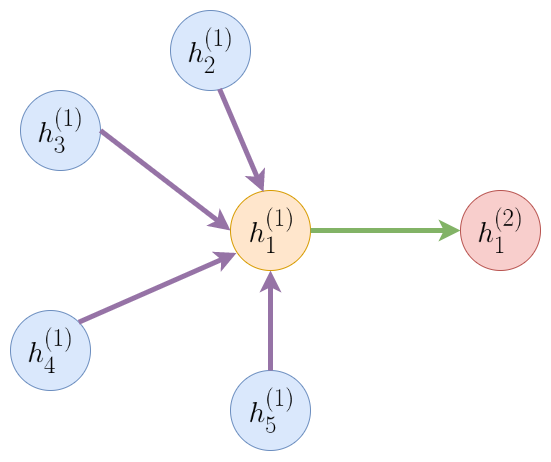
\includegraphics[scale=0.4]{graph_network}
\caption{An example of how message passing is used to exchange the information between nodes.\ The embedding
$h_1^{(1)}$ (marked in orange) of the node $h_1$ is updated by aggregating the embeddings of its
neighbours (marked in blue).\ This process results in the new embedding $h_1^{(2)}$ of the node $h_1$ (marked in red).}
\label{fig:graph_network}
\end{figure}

\subsection{Overview of models}

Over time, researchers have developed multiple ways of modelling aggregating functions $f_k$.\ One of the most
successful approaches, proposed in \cite{gcn_model}, utilises the following aggregation function
$$
H^{(k + 1)} = f_k(H^{(k)}) = \sigma(\tilde{D}^{-\frac{1}{2}} \tilde{A} \tilde{D}^{-\frac{1}{2}} H^{(k)} W^{(k)}))\ ,
$$
where $\sigma$ denotes an activation function, $\tilde{A}$ is the adjacency matrix with added self-loops, $D$ is
a diagonal matrix, such that $D_{ii}$ represents the order of the node $i$ and $W$ is layer-specific trainable
matrix.\ The formula has its mathematical justification, relying on the graph Laplacian.\ From the more intuitive
point of view, $\tilde{D}^{-\frac{1}{2}} \tilde{A} \tilde{D}^{-\frac{1}{2}}$ can be thought of a convolution matrix
that is based on the connectivity of nodes.\ The discussed model is called GCN and has been successfully applied
to many tasks involving graphs.\newline

\noindent The other popular choice for the aggregation functions $f_k$, proposed in \cite{graphsage}, is
Long Short-Term Memory (LSTM).\ In short, LSTM is a recurrent model that can take variable-length
inputs, in parallel reducing the well-known vanishing gradient problem.\ More details of the LSTM model can be found
in \cite{goodfellow_book}.\newline

\noindent Yet another approach is to use a so-called self-attention mechanism that is discussed more deeply in
\textit{Subsection} \ref{subsec:self_attention}.\ In the context of graph neural networks, the above-mentioned
mechanism is used to learn how much attention should be put to a specific neighbour, when receiving its
message.\ Specifically, let $\alpha_{ij} \in [0, 1]$ be a learnable weight, denoting how much attention the node
$i$ should put to its neighbour node $j$ and for non-neighbouring nodes set $\alpha_{ij} = 0.0$.\ Now, let the
aggregation function be defined by the following formula
$$
h_i^{(k + 1)} = f_k(h_i^{(k)}, K) = \sigma(\sum_{h_j^{(k)} \in K} \alpha_{ij}^{(k)} W^{(k)} h_j^{(k)})\ ,
$$
where $K$ denotes the i-th node neighbours, $\sigma$ is an activation function and $W^{(k)}$ is a learnable
matrix.\ Additionally, in order to take into account the current representation of the node $i$, self-connections
are added to the graph.\ The model is optimized to update attention weights $\alpha$ and parameter matrices
$W^{(k)}$, providing additional insights on the importance of specific neighbours.\newline

\section{Reinforcement learning}\label{sec:reinforcement_learning}

Consider a supervised model whose goal is to learn to play a computer game.\ It makes some decisions and based
on them, the environment provides it new states.\ In this situation, the model does not know whether it made the
right decision.\ As a result, it is not provided the ground-truth labels and cannot be supervised.\ This type of
problem, which involves maximizing the long-time reward based on a sequence of decisions, concerns the area of machine
learning called Reinforcement learning.\ Formally, the goal of this learning method is to find a function $\pi$ that
maximizes the so-called utility function
$$
U^{\pi}(s) = \mathbb{E}(\sum_{t=0}^{\infty} \gamma^t R(s_t) | \pi, s = s_0)\ ,
$$
where $\pi$ is a policy function that defines the actions taken by the model, $s_t$ denotes the t-th state
of the game, $R(s_t)$ is a function that assigns a reward to a given state and $\gamma \in (0, 1)$ is a constant
lowering the rewards that are given in the later stage of the game.\ While the policy $\pi$ is deterministic,
the environment can be nondeterministic (e.g.\ the provided state can be based not only on our actions, but also on
how the other player reacts), thus the expected value is applied.\ The naive way of finding the optimal policy would
be to observe that the optimal utility function is defined by
$$
U^{\star}(s) = R(s) + \gamma max_a \sum_{s'} P(s, a, s') U(s')
$$
for each $s \in S$, where $P(s, a, s')$ denotes the probability of landing in the state $s'$, assuming that the
current state is $s$ and that the action $a$ was taken.\ These equations are called the Bellman equations and while
they are not linear, there exist an iterative algorithm for solving the system of such equations.\newline

\noindent In practise, the state space is too large to directly solve the system of Bellman equations.\ The common
solution is to use a function approximating utility function $U$.\ It can be any learnable model and in
particular, the most common choice is to use a neural network.\ In order to learn the approximation function $U$, one
may supervise it by simulating some decisions.\ Instead of performing the exact simulation, it is common to rely on
some approximations that are obtained using Monte Carlo methods.\ These ideas lead to popular Reinforcement learning
algorithms, called Q-learning and Policy Gradients.\ More details behind the presented methods can be
found in \cite{reinforcement_learning_book}.

\section{Transformers}\label{sec:transformers}

Before the rise of transformers, sequence-to-sequence tasks were modelled with recurrent neural
networks.\ These approaches have had many problems as vanishing gradients, causing the quality of models to degrade
for long sequences of inputs.\ While researches have developed many approaches to reduce this issue, training recurrent
models was still inefficient due to their inability to being parallelized.\ Indeed, the main assumption behind
recurrent neural networks is that the outputs of the k-th step cannot be inferred until the outputs of all previous
$k - 1$ steps have been calculated.\ The situation has changed when researchers have proposed
\cite{transformer_model}, introducing the transformer architecture that get rid of all the above-mentioned
issues.\ In the following subsections we define the key components of the proposed transformer architecture and the
extensions that have been developed over time.

\subsection{Self-attention mechanism}\label{subsec:self_attention}

In the abstract form, attention mechanism can be defined as mapping a given query $Q$ and a list of $n$ key-value pairs
$(K, V)$ to output values.\ More formally, we assume that a query $Q$ is a matrix of size $1 \times d_k$, while
a list of keys and their corresponding values form the matrices $K$ and $V$ of size $n \times d_k$.\ While
the attention mechanism can be modelled in many ways, one of the most popular forms is the so-called scaled
dot-product attention
\begin{equation}\label{eq:self_attention}
attention(Q, K, V) = softmax(\frac{Q K^T}{\sqrt{d_k}}) V\ ,
\end{equation}
where $d_k$ is used to scale the computed weights.\ The illustration of the above-defined mechanism is shown in
\textit{Figure} \ref{fig:attention}.\ Intuitively, it computes a convex sum of values, based on the similarity of
the corresponding keys with the query $Q$.\ When $Q = K = V$, the described mechanism is called
self-attention.\ Additionally, one may define attention weights, which in case of the self-attention have the form
$$
\alpha_{ij} = softmax(\frac{Q K^T}{\sqrt{d_k}})_{ij} = softmax(\frac{V V^T}{\sqrt{d_k}})_{ij}\ ,
$$
which indicate how much attention the i-th value (query) puts to the j-th value.\ Indeed, the attention mechanism
was developed in order to learn how much attention should be put into other elements of a sequence.\ Over
time, several extensions of the \textit{Equation} \ref{eq:self_attention} have been proposed to enable the model to
learn better-suited combinations of values $V$ e.g.\
$$
attention(Q, K, V) = softmax(\frac{(Q W_Q) (K W_K)^T}{\sqrt{d_k}}) (V W_V)\ ,
$$
where $W_K, W_V, W_Q$ are learnable matrices mapping keys, values and query, enabling the dot-product between the
query and keys to be computed in the custom space as well as allowing values to be linearly transformed.\newline

\noindent The introduced self-attention mechanism is the key component of the transformer layer that will be discussed
more deeply in \textit{Subsection} \ref{subsec:transformer_encoder_decoder}.\ In particular, it makes use of
multiple attention mechanisms, each learnt using an independent linear transformations
of input keys, values and queries.\ The outputs of all attention mechanisms are concatenated and projected the
final output, using learnable matrix.\ This mechanism is called Multi-Head Attention and is often used instead
of a single attention function.\ Intuitively, this extension allows the model to spread its
attention to different features by adjusting attention weights of each attention head.

\begin{figure}[t]
\centering
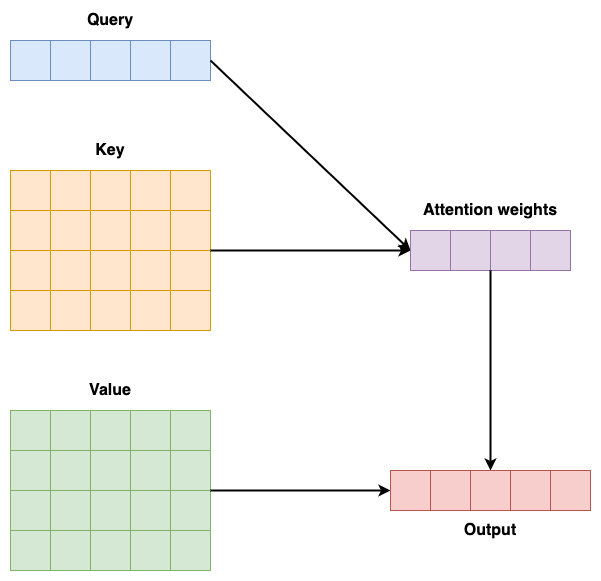
\includegraphics[scale=0.4]{attention}
\caption{An illustration of the attention mechanism.\ In the first stage of the procedure, a query (marked in blue) and
keys (marked in orange) are used to compute attention weights (marked in purple).\ Then, the output (marked in red) is
formed by multiplying a matrix of attention weights with a matrix of values i.e.\ a convex combination of
values is computed.}
\label{fig:attention}
\end{figure}

\subsection{Pointwise feed-forward layer}

While the attention mechanism allows a model to exchange the information between elements of a sequence, the elements
may need to update their representations by itself.\ One of the most intuitive ways to model it, would be to use a few
feed-forward layers, introduced in \textit{Subsection} \ref{subsec:feed_forward}, for each element of the sequence
independently.\ The layer that follows this pattern is called the pointwise feed-forward layer.\ Formally, it takes
a matrix of elements of a sequence and applies a few linear transformations, each followed by an activation
function.\ Importantly, the same transformations are applied to all elements of the sequence.\ This means that a
model is enforced to learn generic transformations, regardless of the characteristics of a specific element.

\subsection{Positional embeddings}\label{subsec:positional_embeddings}

It's a common case that the order of input sequence elements is important.\ For instance, consider a task of
translating a sentence from one language to another.\ In this task, different permutations of words can lead to
various semantics of the whole sentence.\ In order to encode the information about positions of the elements, one
may keep a vector representation of each position and then merge it with a representation of an element on a
specific position.\ Such representation of a position is often referred as a positional embedding.\newline

\noindent The representation of an element can be merged with a position embedding by concatenating their
vectors.\ In case both vectors have the same dimensionality, instead of concatenation, it is common to sum the
corresponding embeddings element-wise.\ One approach to assign a representation to a word is to come up with a
function that could identify each position uniquely.\ In this case, the most popular choice is to use the one
based on different frequencies of some cyclic functions e.g.
$$
PE_{(p, k)} =
\begin{cases}
sin(\frac{p}{100000^{k / d}}) &\text{if $k = 2i$}\\
cos(\frac{p}{100000^{k / d}}) &\text{if $k = 2i + 1$}
\end{cases}\ ,
$$
where $p$ is a position that will be represented by an embedding, $i$ refers to an individual dimension of the
embedding and $d$ denotes the total number of dimensions.\ The other popular choice is to start with random positional
embeddings and update them during the training process, based on the gradient information.

\subsection{Transformer encoder and decoder}\label{subsec:transformer_encoder_decoder}

The introduced multi-head self-attention layer along with the pointwise feed-forward layer form together a
transformer layer, which is illustrated in \textit{Figure} \ref{fig:transformer_layer}.\ The idea behind this layer is
to exchange the information between the elements of a sequence and then update each element independently, leveraging
the two above-mentioned sublayers.\ Additionally, in order to increase the flow of information, skip connections
between the sublayers are applied.\ Specifically, the outputs of the attention sublayer are summed with the original
inputs as well as the outputs of the pointwise sublayer are summed with the outputs of the attention layer.\ This
allows the model to utilise the information contained in the previous layers.\ Besides, it reduces the vanishing
gradients problem i.e\ when the gradient is vanishingly small.\newline

\noindent The transformer encoder is composed of a few stacked transformer layers.\ It takes a sequence of
$n$ input elements, represented by their embeddings (with optionally positional embeddings applied), and returns a
sequence of $n$ embeddings, each representing the corresponding input element in the context of other
elements.\ Similarly to the encoder, the decoder is composed of a few transformer layers.\ The main distinction is
that it takes a sequence of $n$ output elements along with the outputs of the encoder.\ Most commonly,
the outputs of the encoder are injected after a few first transformer layers by summing the output vectors
element-wise.\ The sequence of output elements is often used to provide an information about the previous
outputs.\ For instance, in the machine translation task, it's common to translate a sentence word by word.\ In this
case, the output sequence could contain a partial translation of the input sequence.\newline

\noindent The outputs of the decoder are used to supervise a model.\ The computed gradients are backpropagated
back to the inputs of the encoder, allowing the decoder and encoder to be updated simultaneously.\ In case some
input elements should not be visible by other elements, the corresponding attention weights are set to $0.0$.\ The
introduced layers and techniques form together the original transformer architecture, introduced in
\cite{transformer_model}.\ The model was developed with natural language processing applications in mind, but
can be used in any sequence-to-sequence tasks.

\subsection{Extensions to the original transformer architecture} \label{subsec:transformer_extensions}

Over time, several extensions to the original model were proposed.\ One of the most successful ones include BERT,
introduced in \cite{bert_model}.\ In contrast to the original transformer architecture, it works only
an input sequence.\ This makes it better suited for the tasks, in which the whole output sequence is expected
to be predicted in one pass.\ As a result, the BERT model utilizes only the encoder part of the original transformer
model.\ Additionally, the authors proposed to pretrain the proposed model on two tasks: restoring the masked input
word and predicting the next sentence.\ The proposed approach effectively reduces the training time on the downstream
task, leveraging the knowledge obtained during the pretraining process.\ Furthermore, the model was later
extended in \cite{albert_model} to share the parameters of transformer layers, making it more
parameter-efficient.

\begin{figure}[t]
\centering
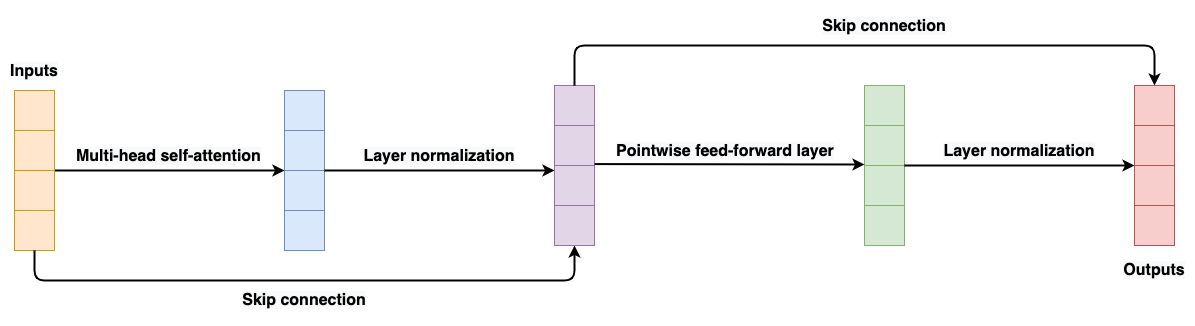
\includegraphics[scale=0.33]{transformer_layer}
\caption{An illustration of the transformer layer.\ Given an input sequence with the encoded positions
(marked in orange), the layer first applies the self-attention mechanism to allow the elements to exchange the
information. Then, the outputs of the attention layer (marked in blue) are normalized and merged with the original
inputs (marked in purple).\ Afterwards, each element of the sequence is transformed independently with the pointwise
feed-forward layer (marked in green). Finally, the elements are normalized and merged with the outputs of the attention
layer, forming the output embeddings (marked in red).}
\label{fig:transformer_layer}
\end{figure}

\noindent Another recently developed extension of the transformer architecture is ELECTRA, introduced
in \cite{electra_model}.\ The authors proposed to train two models in parallel, called generator and
discriminator.\ The generator takes as its input a sequence of elements, with roughly 15\% of random tokens masked
out.\ Its goal is to predict the masked tokens, using a few transformer layers followed by softmax.\ Then, the output
distribution is utilised to sample a token for each position, forming a sequence $s_G$.\ The constructed sequence
$s_G$ is then pushed as an input of the discriminator, which is trained to recognise which tokens are real, considering
the remaining ones as fake.\newline

\noindent At first, the presented ELECTRA model may seem indistinguishable from Generative Adversarial Networks
(GANs), introduced in \cite{gan}.\ However, if one delves into the details, there are several differences.\ Firstly,
in the case ELECTRA, the gradients of the generator and the discriminator are disjoint, causing the
information not to flow from one model the other one one.\ The other distinction is that the generator
is trained to generate real samples that are leveraged by the discriminator, unlike in GANs where the
discriminator tries to generate fake samples that are pushed as inputs to the generator.\ Lastly, after the
training procedure is finished, ELECTRA throws out the generator instead of the discriminator.\ In particular, the
whole procedure can be treated as the form of pretraining as the discriminator is further used to train the model on the
downstream task.

\section{Models proposed for the graph completion problem}\label{sec:background_models}

In this section, we will present the related work on the knowledge graph completion problem.\ The methods will be
presented from the simplest context-free ones that are based on convolutional networks to the more advanced
contextualised ones based on reinforcement learning or graph neural networks.\ While in the recent few years hundreds of
different methods have been developed, we chose the ones that provided a significant quality boost compared to their
predecessors.\ In parallel, we omit the methods that report inflated quality results due to improper evaluation
protocol.

\subsection{Context-free methods}

One of the most influential idea to tackle the problem of knowledge graph completion, was to represent entities and
relations by low-dimensional continuous vectors, called embeddings.\ The most known model applying this idea is
\textbf{TransE}, introduced in \cite{transe_model}.\ The authors proposed to
start with random embeddings of entities and relations, then iteratively update them by optimizing the model
with the following loss function
$$
L(h, r, t, h', t') = max(0, ||h + r - t||_2 - ||h' + r - t'||_2 + \gamma)\ ,
$$
where $(h, r, t)$ represents a (positive) triple that belongs to the knowledge graph, while a (negative) triple
$(h', r, t')$ is formed by replacing either $h$ or $t$, with a random entity.\ Intuitively, this model tries to
rotate vectors representing entities and relations in a way that the norm of the expression $||h + r - t||_2$ is higher
for positive triples than for negative triples.\ Additionally, the margin parameter $\gamma$ controls how high the
difference between the norms should be in order to have $0.0$ loss.\ Interestingly, the discussed architecture can be
treated as a 1D convolution layer of $D \times 3$ image with fixed $(1, 1, -1)$ kernel.\ The TransE model was
further extended to \textbf{STransE} in \cite{stranse_model} to allow relation-specific embeddings of entities.\ More
formally, the authors replaced the expression $||h + r - t||_2$ with $||W_{h,r} h + r - W_{t,r} t||_2$, allowing more
flexible representations.\newline

\noindent In the recent years, many improvements to the TransE model have been proposed.\ In particular, several
methods applying convolutional layers on top of embeddings have been developed.\ For instance, in \cite{conve_model} the
authors proposed \textbf{ConvE} model that concatenates the known head/tail entity embedding with the relation
embedding, forming $D \times 2$ image.\ After that, a convolutional layer, followed by a feed-forward projection layer,
are applied to obtain the output embedding $e_o$ of dimensionality $D$.\ Finally, a dot-product between $e_o$ and each
entity $e \in E$ is computed to find the most similar entity to $e_o$.\ The model is supervised by a softmax function
that is used to maximize the similarity between $e_o$ and the-ground truth tail/head entity that should be
predicted.\ In order to allow the model to distinguish between input and output relations, separate
relation embeddings are used for head and tail entities.\ The model not only optimizes the weights of intermediate
layers, but also finetunes entity and relation embeddings.\ Additionally, it makes use of Dropout and Label
Smoothing to prevent overfitting.

\subsection{Context-based methods}

With the rise of machine learning models operating on graphs, several context-based methods for knowledge graph
completion have been proposed.\ For instance, in \cite{sacn_model} the authors introduced the \textbf{SACN} model,
leveraging custom WGCN layer
$$
h_i^{(k + 1)} = \sigma(\sum_{j \in N(i)} \alpha_{r(i, j)} g(h_i^{(k)}, h_j^{(k)}))\ ,
$$
where $g$ specifies how to incorporate neighboring information and $r(i, j)$ denotes the relation that connects the i-th
node with the j-th node.\ Intuitively, the idea is to make it possible for each relation to focus on different parts
of the neighbouring embeddings.\ The proposed model is composed of a few WGCN layers that collect the information from
the neighbourhood, forming the embedding of the source entity $e_s$.\ Then, a convolutional network is applied on top of
the aggregated embedding $e_s$ and input relation embedding, with the goal to predict the target entity.\ In particular,
this architecture is similar to the ConvE model, except the fact that the embedding of the source entity is formed by
aggregating neighbouring embeddings.\newline

\noindent The downside of the model discussed above is that the representations of relations are not updated by the
graph neural network itself.\ In particular, the only way the aggregation function can leverage relation-specific
information is by adjusting attention weights.\ The other approach is presented in the \textbf{CompGCN} model,
introduced in \cite{comp_gcn_model}, where the representations of relations are used directly by the graph neural
network.\ More precisely, the authors defined the aggregation function
$$
h_i^{(k + 1)} = \sigma(\sum_{j \in N(i)} W_{\lambda(r)} g(h_j^{(k)}, r_j^{(k)}))\ ,
$$
where $r_j^{(k)}$ denotes the representation of the j-th relation in the context of the k-th aggregation function and
$\lambda(r)$ is used to select one of three matrices, depending on the type of relation $r$.\ Specifically, the
matrix $W_O^{(k)}$ is used for relations originally contained in the knowledge graph, $W_I^{(k)}$ is used for added
inverse relations and $W_S^{(k)}$ is used for self-loops.\ This allows the information to flow in both sides, while
keeping the number of model's parameters low.\ Additionally, the relation embeddings are transformed after each layer
$$
r_i^{(k + 1)} = \tilde{W} r_i^{(k)}\ ,
$$
which makes the aggregation functions more flexible.\ Finally, the authors tested the proposed CompGCN model with
multiple scoring functions applied on top of aggregated embeddings, including TransE and ConvE.\newline

\noindent The other interesting approach was taken in \cite{go_for_a_walk_model}, introducing the \textbf{MINERVA}
model.\ The authors proposed to learn it to walk though a graph in order to find a missing head or tail
entity.\ More specifically, given a source entity and a relation, the goal is to take a sequence of decisions that
will lead to the target entity, where in each step the model can go to one of its neighbours or remain in the current
node.\ After a fixed number of steps, in case the model lands in the target entity, it is given a reward.\ Additionally,
in order to increase the awareness about the visited nodes, the history is included in the model's state.


\numberedchapter{Developed methods}\label{chapter:developed_methods}

In the following sections we will discuss our transformer-based approach in depth.\ We will start by introducing the
main components, forming our context-free architecture.\ Then, we will go through the developed extensions, which
add graph context to our model.\ Lastly, we will define the models that were selected for further
experiments discussed in \textit{Chapter} \ref{chapter:experiments}.

\section{Context-free transformer architecture}\label{sec:context_free_model}

Our model assigns latent representations (embeddings) to each entity and relation of a given knowledge
graph.\ Additionally, we leverage positional embeddings discussed in \ref{subsec:positional_embeddings} and
model-specific embeddings of special tokens.\ We refer to the above-mentioned objects as tokens.\ In particular, we
keep all tokens in one large vocabulary $V$ and their embeddings in a matrix $T$ of size $|V| \times D$, where $D$
denotes the dimensionality of one token.\ The embedding of a token can be thought of its learnable
representation.\ The details on how we initialize and train token embeddings are
included \textit{Subsection} \ref{subsec:token_embeddings}.\newline

\noindent The developed architecture takes as its input a batch samples, where each sample is composed of a sequence of
input tokens.\ In case of context-free model, all input sequences are of length 3, while in other models different
training batches may contain sequences of different lengths.\ Nevertheless, all input sequences of a specific
training batch are expected to be of the same length.\ Each token is transformed to the corresponding embedding and then
several transformer layers, introduced in \textit{Subsection} \ref{subsec:transformer_encoder_decoder}, are applied to
form the output sequence.\ This process can be interpreted as exchanging information between tokens, where each token
can extract information from all other tokens and in particular, it can choose which information is useful using
self-attention mechanism.\ The output sequence of contextualised tokens is used to supervise the model.\ The high-level
overview of our model is shown in \textit{Figure} \ref{fig:high_level_view_of_our_model}.\ The details of
sequence-to-sequence mapping component as well as loss functions are discussed more deeply in \textit{Subsection}
\ref{subsec:sequence_to_sequence_mapping} and \textit{Subsection} \ref{subsec:transformer_loss_functions}
respectively.\ Besides it, we highlight the importance of normalization layers in \textit{Subsection}
\ref{subsec:normalization_layers}.\newline

\noindent In case of context-free architecture, input tokens are partially masked triplets, representing edges
contained in the training dataset.\ More specifically, for a given training triple $(h, r, t)$, we mask out either head
entity $h$ or tail entity $t$.\ This forms either $([mask], r, t)$ or $(h, r, [mask])$ sequence, where $[mask]$ is a
special token with a learnable embedding.\ In particular, for each edge we form both sequences and randomly shuffle all
formed samples.\ After transforming tokens to their corresponding embeddings and applying sequence-to-sequence
component, $(h_c, r_c, t_c)$ sequence of embeddings is obtained.\ We interpret each embedding as a contextualised
representation of the corresponding input token.\ Particularly, the model is supervised in a way that the output token
on a position matching $[mask]$ input token is close to the $h_e$ embedding/$h_t$ embedding of the masked head/tail
entity.\ The closer both embeddings are, the better the model is.\ Both variants of the masked head and tail entity
are presented in \textit{Figure} \ref{fig:context_free_model}.

\begin{figure}[t]
\centering
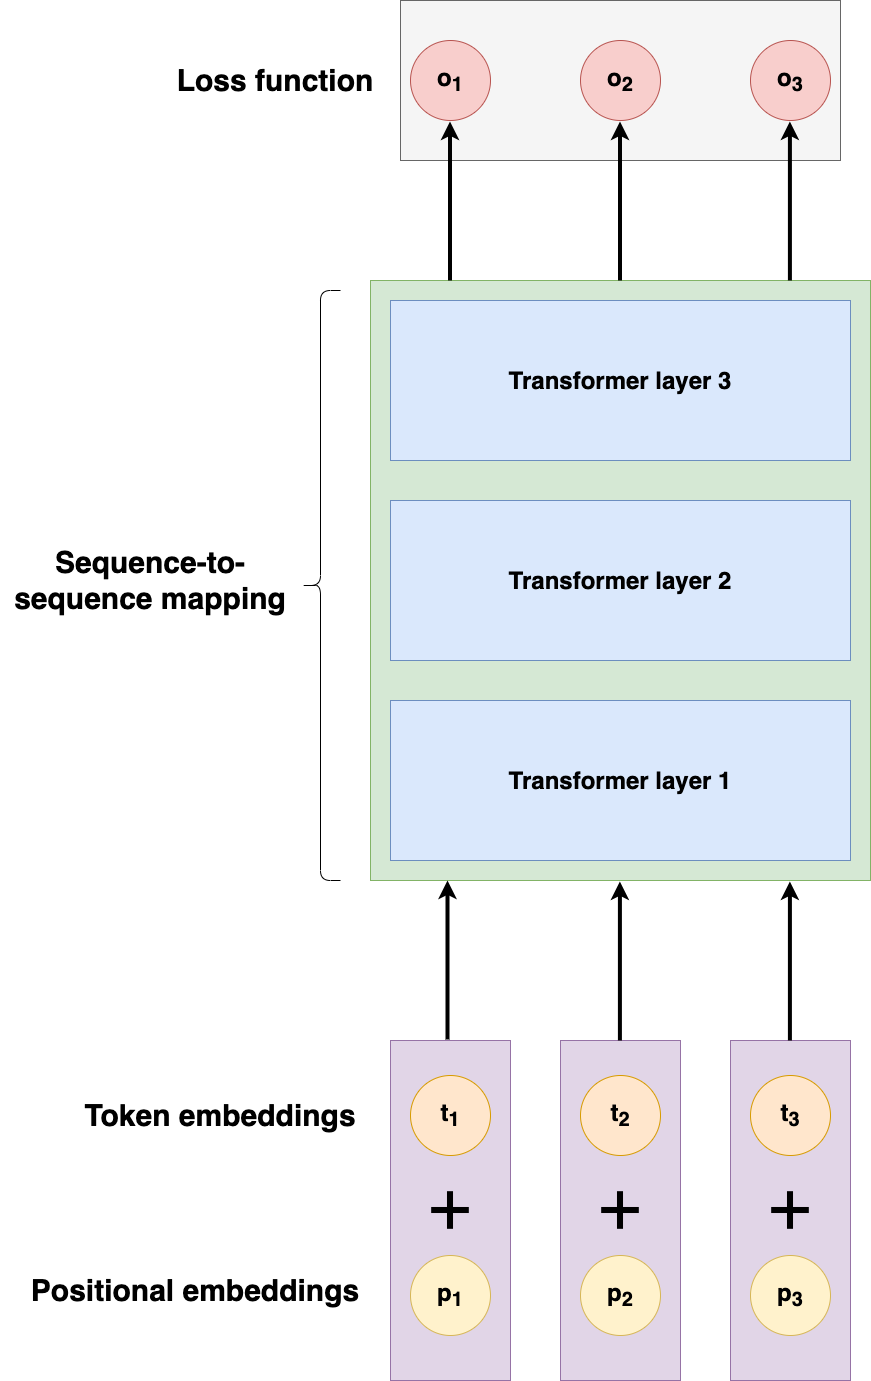
\includegraphics[scale=0.23]{high_level_view_of_our_model}
\caption{A high-level overview of our architecture.\ First, input tokens are mapped to their corresponding
embeddings (marked in orange) and summed element-wise with positional embeddings (marked in yellow).\ The formed
embeddings are marked in purple.\ Then, a few transformer layers (marked in blue), forming together sequence-to-sequence
component (marked in green), are applied to map input sequence to output tokens.\ The outputs of the last layer
(marked in red) are then passed to the loss function component (marked in gray) that supervise the whole model.}
\label{fig:high_level_view_of_our_model}
\end{figure}

\begin{figure}[t]
\centering
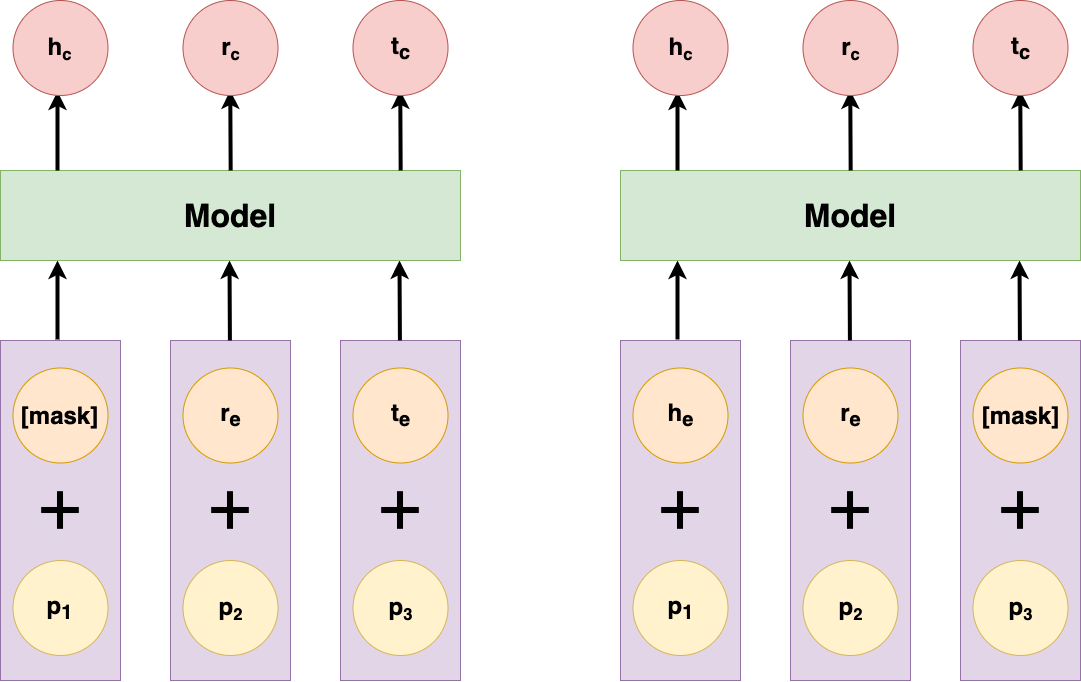
\includegraphics[scale=0.25]{context_free_model}
\caption{An illustration of input and output sequences of the developed context-free model.\ In the first case
(on the left), head entity is masked out, while relation and tail entity embeddings are pushed to the model.\ The model
is expected to restore the masked head entity.\ In the other case (on the right), tail entity is masked out and the
model is learnt to restore it, given embeddings of relation and head entity.}
\label{fig:context_free_model}
\end{figure}

\subsection{Initialising and training token embeddings}\label{subsec:token_embeddings}

We have explored various approaches for embeddings initialization.\ We found that initialising embeddings of
all tokens with random values provides the best results.\ Importantly, the initialized values should in a small range
$[-0.05, 0.05]$, otherwise the network loses its capability to learn anything.\ We also explored several
initialization distributions, including uniform and normal distribution.\ We found that in case of our models, the
truncated normal distribution, which bounds normally distributed variable from below and above, provides the best
quality.\ Besides it, we noticed that applying dropout layer discussed in \ref{subsec:overfitting} significantly
reduces overfitting of our model.\newline

\noindent For entities and relations, we also experimented with initialization by pretrained embeddings.\ More
specifically, we trained TransE, ConvE models and then utilised trained representations to initialize our model.\ In
parallel, we initialized special token and positional embeddings with random values.\ As
the dimensionality of the learnt TransE embeddings is lower than the dimensionality of our model's embeddings, we
filled the remaining parts of embeddings with random values.\ Additionally, as the pretrained embeddings are in a wide
range, which could harm the learning capability of our model, we experimented with scaling them by a constant
factor.\ Nevertheless, during our experiments, we didn't notice any quality boost by using the above-discussed
initialization techniques.\ Therefore, we decided to stick with random initialization approach, which we find simple
and effective.\newline

\noindent In our experiments, we also tested fixed-function initialization of positional embeddings, discussed in
\textit{Subsection} \ref{subsec:positional_embeddings}.\ In this case, the embeddings are fixed during the whole
training procedure.\ We found that this initialization technique affects the quality of the trained models badly.


\subsection{Sequence-to-sequence mapping}\label{subsec:sequence_to_sequence_mapping}

Regardless of the number of input tokens, several transformer layers are applied on top of all of them.\ In the
default setting each transformer layer contains independent parameters.\ We also experimented with sharing all
corresponding parameters between transformer layers, forming an architecture similar to ALBERT that was discussed
in \textit{Subsection} \ref{subsec:transformer_extensions}.\ We achieve similar quality of models in both
settings.\ The parameter-sharing approach might be preferred in real applications as it has a few million less
parameters.\ Nevertheless, more than half of the total number of parameters come from token embeddings.\newline

\noindent Our experiments showed that the best performance is achieved when 6-12 transformer layers are
applied.\ Importantly, each layer utilises multi-head attention mechanism discussed in \textit{Subsection}
\ref{subsec:self_attention}.\ We found that at least 4 attention heads are needed to achieve the best
quality of models.\ We also experimented with attention head dimension $D_a$ and pointwise feed-forward layer
dimension $D_p$.\ Our analysis showed the the best quality is attained when $2 D_a = D_p = 512$.\ Lastly, we noticed
that adding dropout layers before the components computing attention weights and before pointwise feed-forward layers,
slightly reduces overfitting.\ Therefore, we include dropout layers in all our models.


\subsection{Loss functions and model optimization}\label{subsec:transformer_loss_functions}

The goal of our context-free model is to restore the masked head/tail entity.\ To compute similarities between
each entity $e_i \in E$ and the produced embedding $p$, we use dot product.\ More precisely, we compute
$$
e_i \cdot p = \sum\limits_{j=1}^{D} e_{ij} p_j\ ,
$$
where $p = h_c$ if head entity was masked out and $p = t_c$ in case tail entity was masked out.\ As a result, a vector
$t$ is formed, such that $t_i$ indicates a score of the i-th entity.\ Then, we apply softmax activation function on
$t$ to obtain a probability distribution $\tilde{t}$.\ Lastly, the cross-entropy loss function, discussed in
\textit{Subsection} \ref{subsec:loss_functions}, is computed between $\tilde{t}$ and a vector encoding an index of
the masked head/tail entity.\ The computed loss is utilised to compute gradients of all model's parameters, including
token embeddings.\ The optimization process is taken by Adam optimizer discussed in \textit{Subsection}
\ref{subsec:optimization}. \newline

\noindent During our experiments, we found that several optimization details play a crucial role in boosting the
quality of our models.\ First of all, we apply label smoothing discussed in
\textit{Subsection} \ref{subsec:overfitting}.\ We find that it greatly reduces overfitting and in particular, setting
label smoothing parameter $s \in (0, 1)$ to a high value $s > 0.5$ significantly increases the performance of our
models on unseen samples.\ The exact optimal value of $s$ is dataset-dependent, therefore it is finetuned for each
experiment.\ The other important specific of our models is the gradient computation.\ On this point, the training
process is more stable when softmax activation is computed along with cross entropy loss function, with the simplified
formula.\ In our experiments, we noticed that it makes the gradient computation more precise and as a result the
trained models converge faster.\ We also noticed that it impacts the final quality metrics measured on unseen
samples.\newline

\noindent We also experimented with other optimization variants.\ In particular, we discovered that an
alternative approach is to replace softmax activation function with sigmoid activation defined using the formula
$$
\sigma(x) = \frac{1}{1 + e^{-x}}\ .
$$
In this setting, each entity is assigned a probability $\tilde{t} \in [0, 1]$ independently.\ In our experiments, we
found that models trained in this way attain similar quality to when the softmax function is used.\ The other tested
approach includes encoding all matching head/tail entities in one training sample.\ In this case, a vector encoding
ground-truth entities contains multiple $1.0$ values and the model is penalized by all of these entries at
once.\ Nevertheless, we didn't notice any quality boost when using this approach.

\subsection{Normalization layers}\label{subsec:normalization_layers}

In our experiments, we also tested the impact of applying normalization layers discussed in
\textit{Subsection} \ref{subsec:normalization_layers}.\ We found that including them in our models
has a positive impact on the quality of our models.\ More specifically, we put normalization layers in 3 places, namely
straight on top embeddings, after attention layers and after pointwise feed-forward layers.\ Including all of the
above-mentioned layers have a strong positive impact on the final models' quality.\ Additionally, we noticed that
using layer normalization over batch normalization is beneficial for our models.\ Lastly, we experimented with the
placement of normalization layers inside transformer blocks, discussed in
\cite{layer_normalization_in_transformers}.\ Nevertheless, we discovered that placing normalization layers in
different parts of the transformer blocks doesn't have much impact on our models.

\section{Adding context to the developed architecture}\label{sec:context_models}

In the following section we will discuss the extensions developed to improve the context-free model.\ Particularly, we
will focus on different approaches to utilise context of a graph representing training dataset.\ We reuse all of the
components discussed in \textit{Section} \ref{sec:context_free_model}, including developed layers, overfitting
prevention methods and loss functions.\ Nevertheless, we finetune parameters of each extended model separately as
each of them has different characteristics.\ While this section covers only methods of putting additional context
into the developed model, in \textit{Section} \ref{sec:training_strategies} we discuss several strategies to train the
extended models.\ Finally, we put everything together in \textit{Section} \ref{sec:selected_models}, providing the most
successful models.

\subsection{Path-based context}

The most natural approach to provide the context information to our model is to utilise nodes neighbouring with a given
source entity.\ The simplest way of applying this idea is to add one random neighbour along with a relation connecting
it with the source entity, forming a path $(e_h, r_h, e_p, r_t, e_t)$, where either $e_h$ or $e_t$ is masked
out.\ An illustration presenting this approach is shown in \textit{Figure} \ref{fig:path_based_model}.\ In our
experiments, we draw several millions of paths, each forming one sample with missing head and one sample with missing
tail.\ We also find it beneficial for our models to randomly mask out intermediate entity $e_p$.\ It enforces the
model not to memorize edges that are contained in constructed paths.\ Additionally, we experimented with paths longer
than 2, nevertheless we didn't observe any quality boost by doing so.\newline

\begin{figure}[h!]
\centering
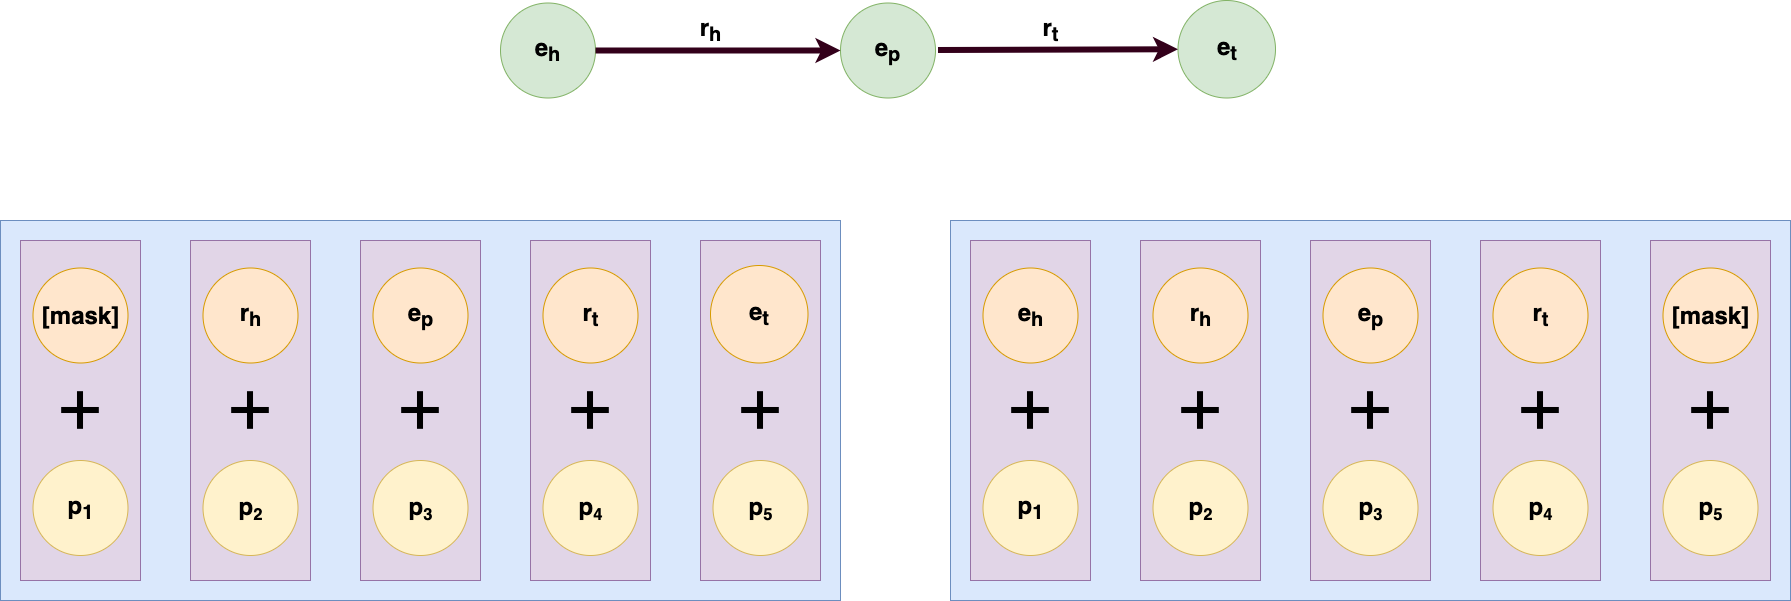
\includegraphics[scale=0.22]{path_based_model}
\caption{An illustration of how path-based context information is used during the training process.\ The top part
of the figure presents a path of length 2 extracted from the knowledge graph, while the bottom part shows corresponding
training samples.\ The bottom-left part illustrates a training sample with masked head entity.\ Similarly, the
bottom-right part illustrates a training with masked tail entity.\ The entity $e_p$ is randomly masked out with a
probability defined by a hyperparameter.}
\label{fig:path_based_model}
\end{figure}

\subsection{Relation-based context}

Another idea is to learn the model to predict a relation that connects given head and tail entities.\ This approach is
illustrated in \textit{Figure} \ref{fig:relation_based_model}.\ Intuitively, adding relation prediction task to
optimize our model can help it in understanding different relations, leading the model to learn better
representations.\ This knowledge can transfer to our final task of predicting a missing head/tail
entity.\ As in this case the goal of the model is to restore a relation, similarities used for the loss computation
are computed between the produced embedding and each relation $r_i \in R$.\newline

\begin{figure}[h!]
\centering
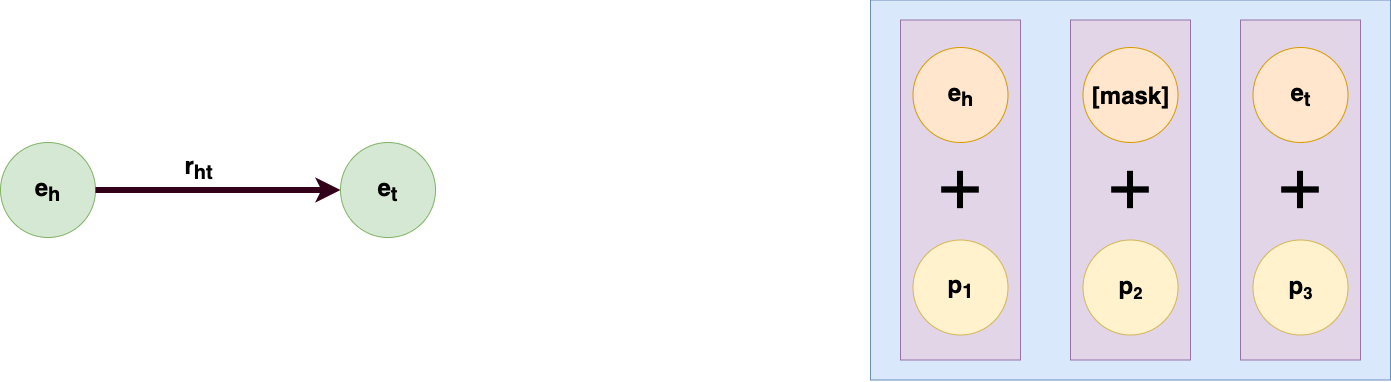
\includegraphics[scale=0.25]{relation_based_model}
\caption{An example of how our models are learnt to predict relations.\ The left part of the figure shows the edge
extracted from the knowledge graph, while the right side presents a training sample that corresponds to the extracted
edge.}
\label{fig:relation_based_model}
\end{figure}

\subsection{Neighbours-based context}

We also experiment with adding a larger context to our model.\ More specifically, we encode input edges/output edges
(or both) of the source entity.\ For each training sample, we use a fixed number of edges $N$.\ In case the source
entity contains more than $N$ neighbours, random $N$ neighbours are sampled.\ On the other hand, if the source entity
contains less than $N$ neighbours, special tokens are put in the corresponding places of the input sequence.\ As the
order of neighbours is not intended to impact the model's predictions, their positional embeddings are shared.\ The case
when the source entity corresponds to the tail entity, while the head entity is masked out is shown
in \textit{Figure} \ref{fig:neighbours_based_model_input_variant}.\ Similarly, the other case of tail entity masked out
is illustrated in Figure \ref{fig:neighbours_based_model_output_variant}.\newline

\noindent During our experiments, we applied several modifications of adding neighbours-based context to our
model.\ First of all, we randomly mask out the source entity to assure that the model does not memorize edges encoded
in a given input sequence.\ Secondly, in case both input and output edges are included, we randomly mask out edges
contained in one of this category.\ Lastly, we observed a positive impact of keeping the sampled neighbourhood of
a given source entity fixed during the whole optimization process as well during the inference.\ In particular, it
has a high impact on predictions of samples for which the source entity contains very large number of neighbours.

\begin{figure}[h!]
\centering
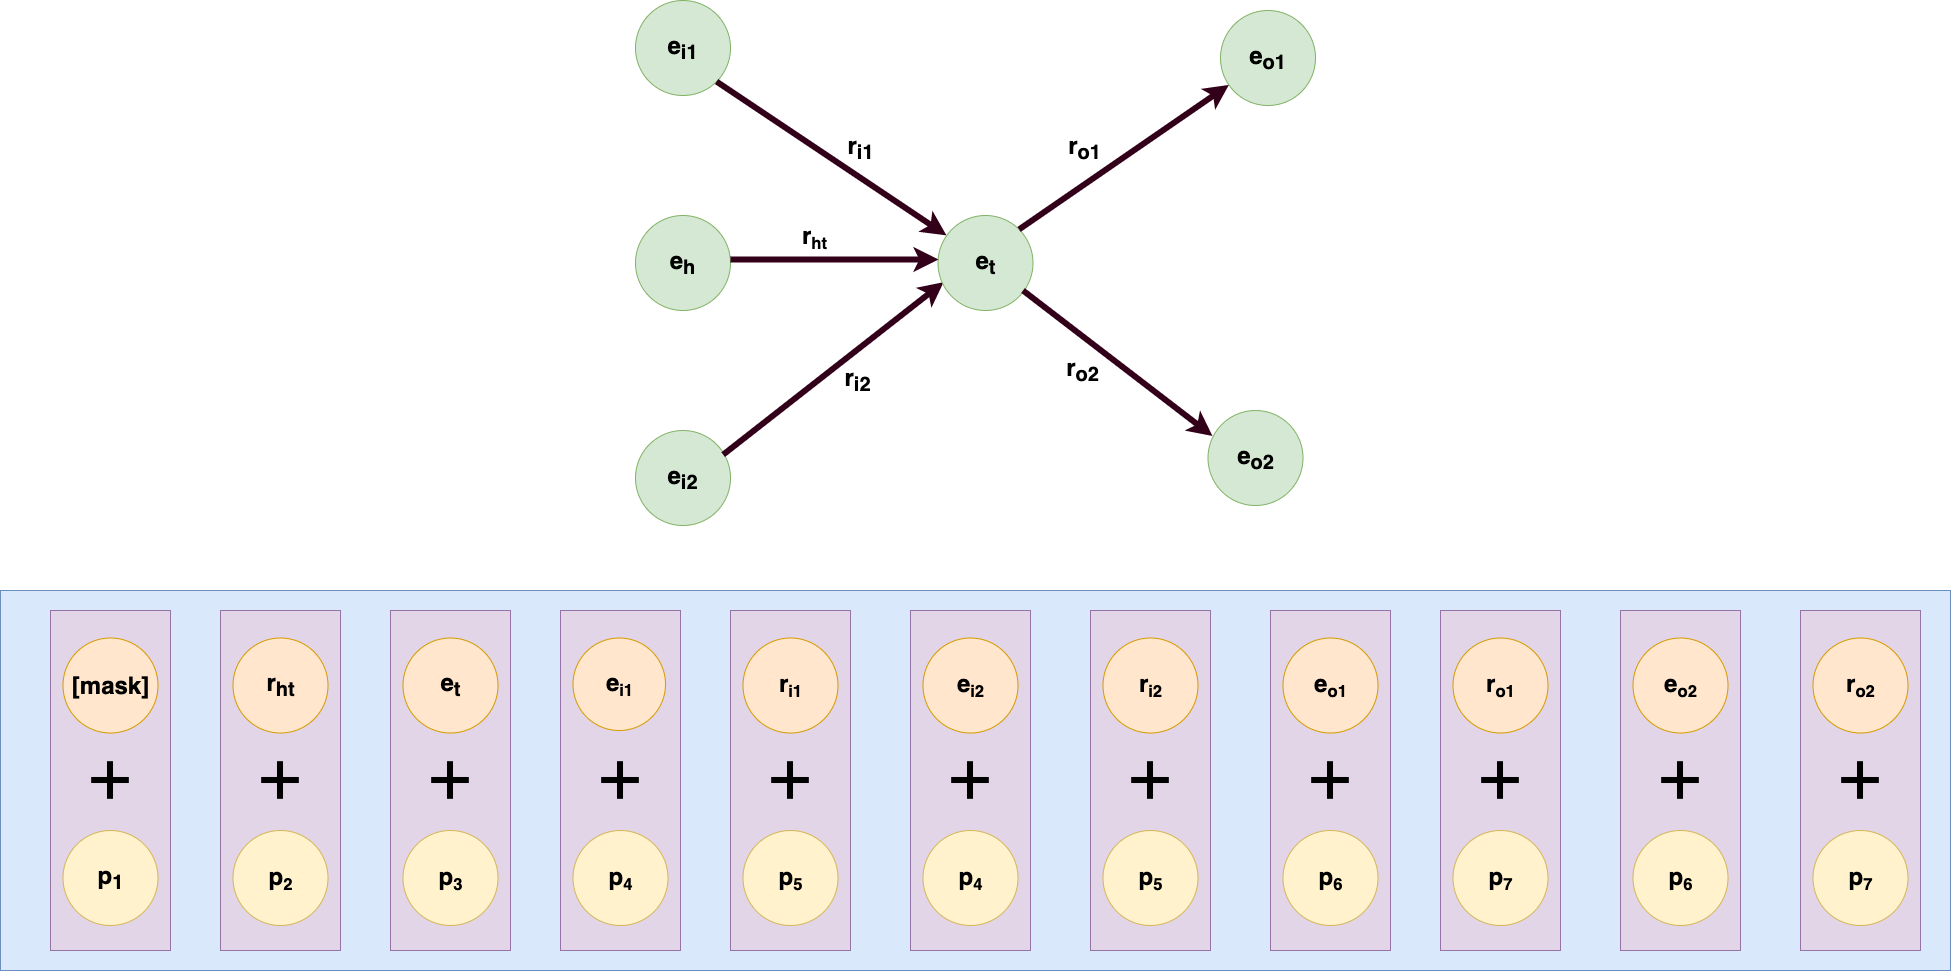
\includegraphics[scale=0.2]{neighbours_based_model_input_variant}
\caption{An example of how the context of input and output neighbours is utilised to produce a training sample with
masked head entity.\ The top part of the figure presents a subgraph containing $(e_h, r_{ht}, e_t)$ edge.\ The bottom
part illustrates the subgraph encoded into input sequence taken by the model.}
\label{fig:neighbours_based_model_input_variant}
\end{figure}

\begin{figure}[h!]
\centering
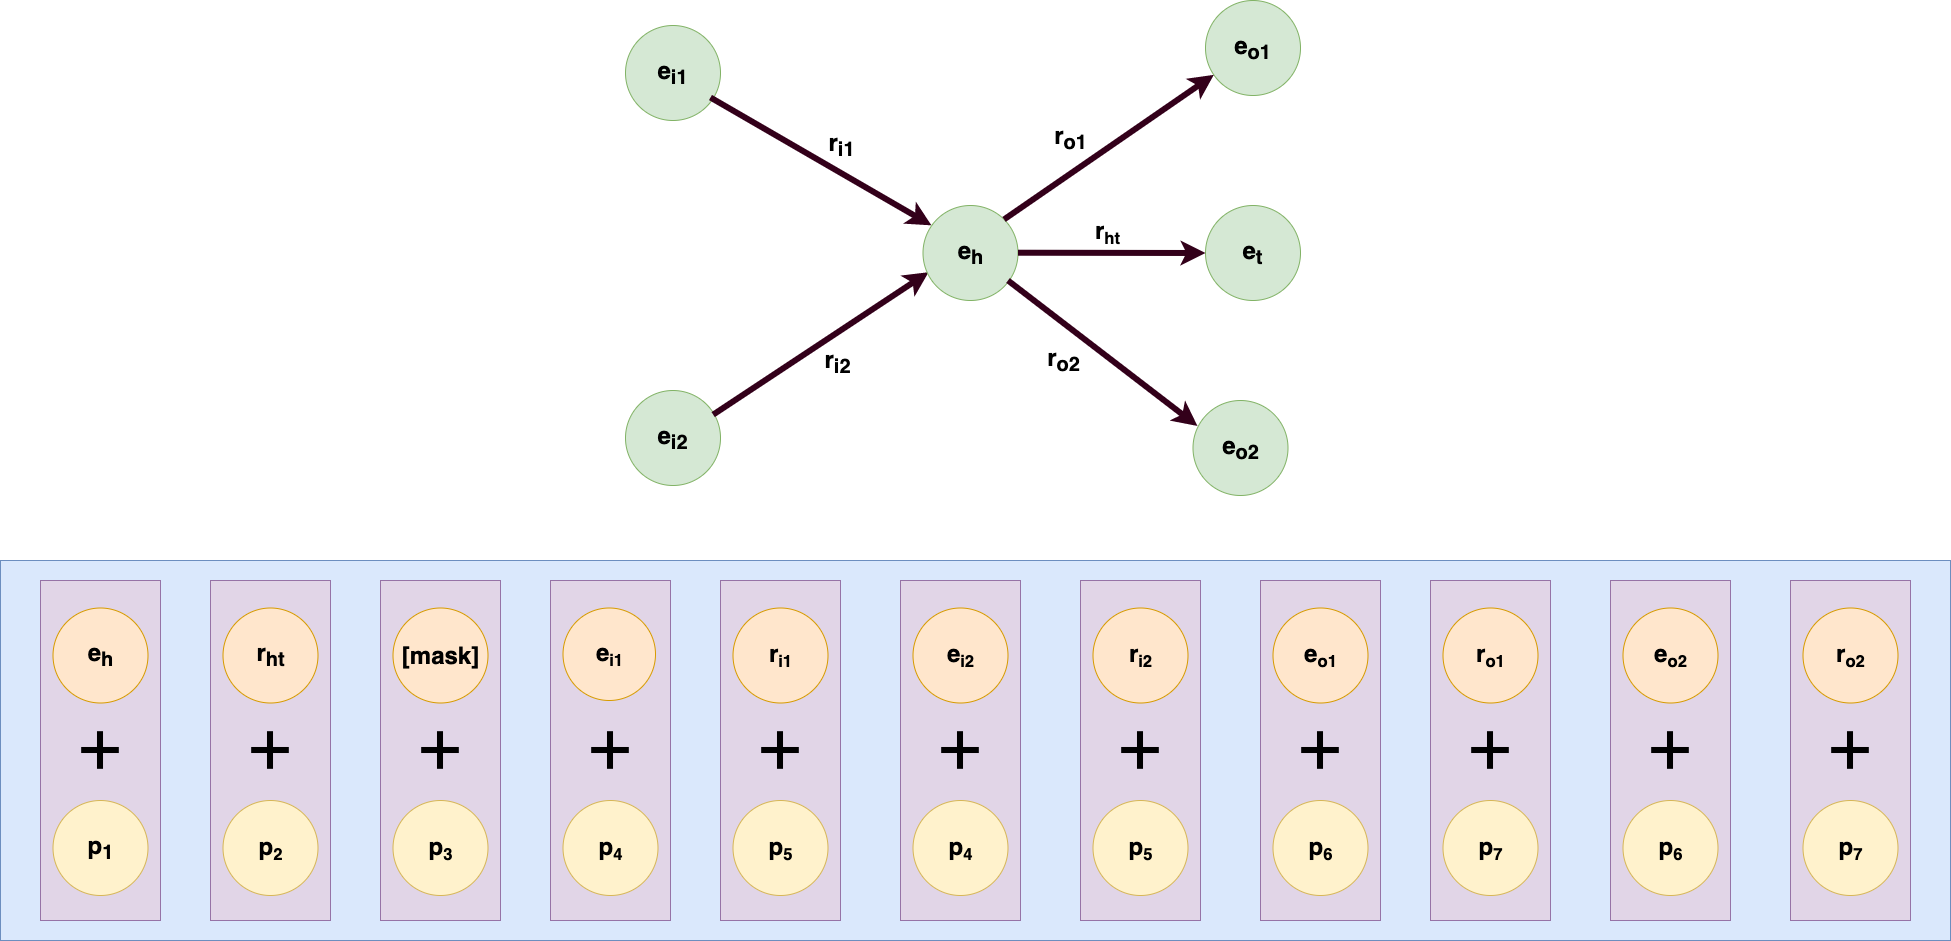
\includegraphics[scale=0.2]{neighbours_based_model_output_variant}
\caption{An illustration of how the context of input and output neighbours is used to form a training sample with
masked tail entity.\ The top part of the figure shows a subgraph containing $(e_h, r_{ht}, e_t)$ edge.\ The bottom
part presents the subgraph encoded into input sequence taken by the model.}
\label{fig:neighbours_based_model_output_variant}
\end{figure}

\subsection{Similarity-based context}

Our analysis of two benchmark datasets showed that many entities of a specific knowledge graph share common
characteristics.\ In particular, many of them have common neighbours connected by the same relation.\ Inspired by
this observation, we decided to collect similar entities and leverage these similarities during the optimization
process of our model.\newline

\noindent In order to formulate similarities, for each entity $e_k$ we define a set of output
relations $R_O(e_k) = \{r_1, \dots, r_{M_k}\}$ (analogically a set of input relations) contained in the training
dataset.\ We ignore the information of how many times a specific relation occurs in edges outcoming from
$e_k$.\ We find two entities $e_k, e_l$ similar if their sets of output edges $R_O(e_k)$ and $R_O(e_l)$ are
similar.\ While there are many ways to formulate the similarity of sets, we use Jaccard index, which is defined using
the formula
$$
J_O(e_k, e_l) = \frac{|R_O(e_k) \cap R_O(e_l)|}{|R_O(e_k) \cup R_O(e_l)|}
$$
Based on the above definition, we formulate the distance between two entities as
$$
D_O(e_k, e_l) = 1 - J_O(e_k, e_l)\ .
$$
For each entity $e_k$, we keep $N$ entities that are the closest ones in the metric space defined by
$D_O(e_k, e_l)$, forming $S_O(e_k)$ sets.\ To avoid the computation of similarities between each pair of entities
explicitly, we use Ball Tree data structure that splits the space recursively in order to keep similar entities
in neighbouring subspaces.\ Analogously, similar entities with respect to input edges are selected, forming
$S_I(e_k)$ sets.\newline

\noindent Now, we will focus on how we leverage $S_O(e_k)$ and $S_I(e_k)$ sets to add context information to our
model.\ Our idea is to find edges that might be similar to a given, partially masked $(e_h, r_{ht}, e_t)$
edge.\ In case the head entity $e_h$ is masked out, we first extract entities similar to $e_t$ according to the
set $S_I(e_t)$.\ Then, we sample $K$ edges $(e_{i(k)}, r_{ht}, e_{o(k)})$, such that
$e_{o(k)} \in S_I(e_t)$.\ Intuitively, $e_{i(k)}$ might be a good candidate for being the masked head entity $e_h$.\ As
a result, it makes sense to contain this information in the input sequence pushed to our model.\ The way of encoding
this information is shown in \textit{Figure} \ref{fig:similarity_based_model_input_variant}.\newline

\noindent In case of the masked tail entity, the extraction of similar edges is analogous.\ The main difference is
that the set $S_O(e_h)$ is used to extract searched entities.\ The other significant difference is that edges
$(e_{i(k)}, r_{ht}, e_{o(k)})$ are samples with the $e_{i(k)} \in S_O(e_h)$ constraint.\ The discussed variant is
illustrated in \textit{Figure} \ref{fig:similarity_based_model_output_variant}.\newline

\noindent During our experiments, we finetune the parameter controlling the number of similar entities pushed to
the model.\ We also experimented with removing entities that are similar to the source entity from the input
sequence.\ In this case, input sequences contain only entities that are candidates for being the masked out
entity.\ Nevertheless, we did not observe any performance gains or losses by applying this modification.\ Lastly,
as sampled context edges are permutation-invariant, we share their positional embeddings, what actually impacts
the performance of our model positively.


\begin{figure}[h!]
\centering
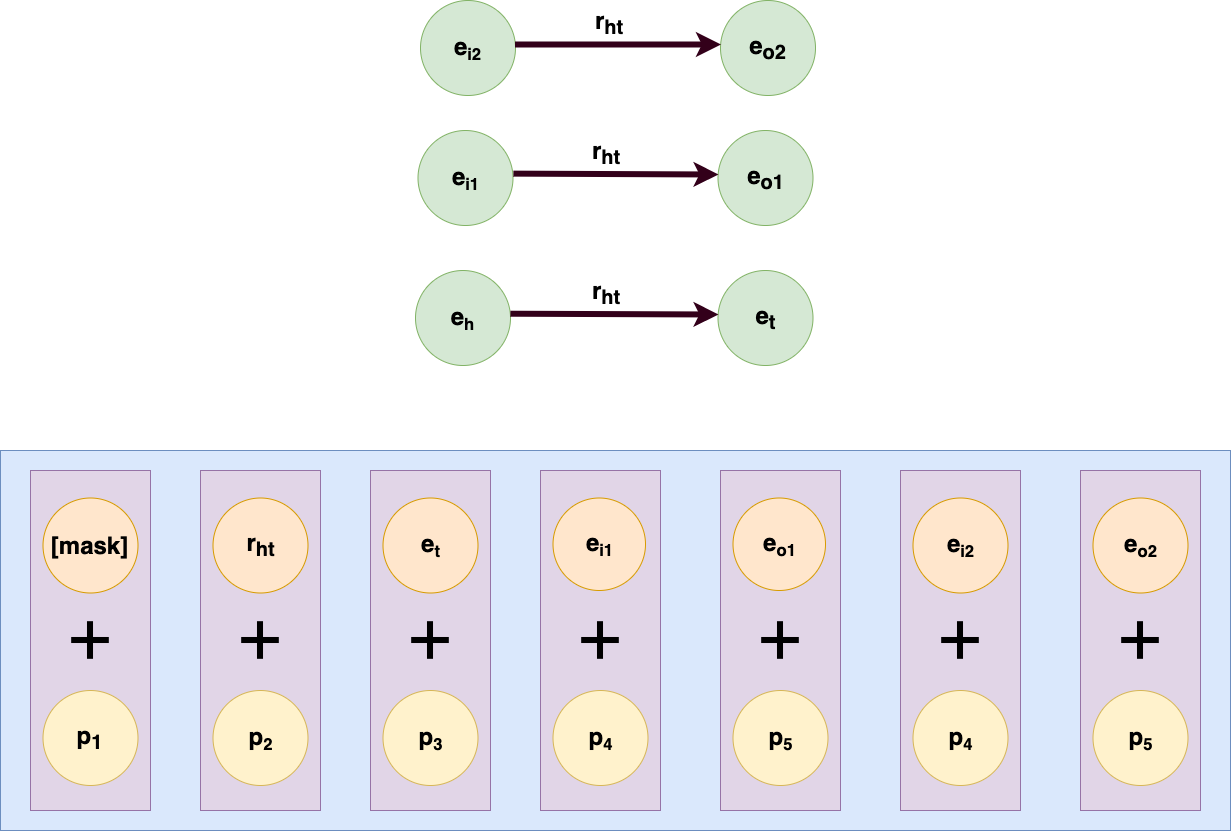
\includegraphics[scale=0.27]{similarity_based_model_input_variant}
\caption{An example of how similar entities are utilised to form a training sample with a missing head
entity.\ The top part of the figure presents a partially masked edge $(e_h, r_{ht}, e_t)$ along with sampled edges,
such that $e_{o1}$, $e_{o2}$ entities are similar to $e_t$. The bottom part illustrates how this information is
encoded into input sequence pushed to the model.\newline
}
\label{fig:similarity_based_model_input_variant}
\end{figure}

\begin{figure}[h!]
\centering
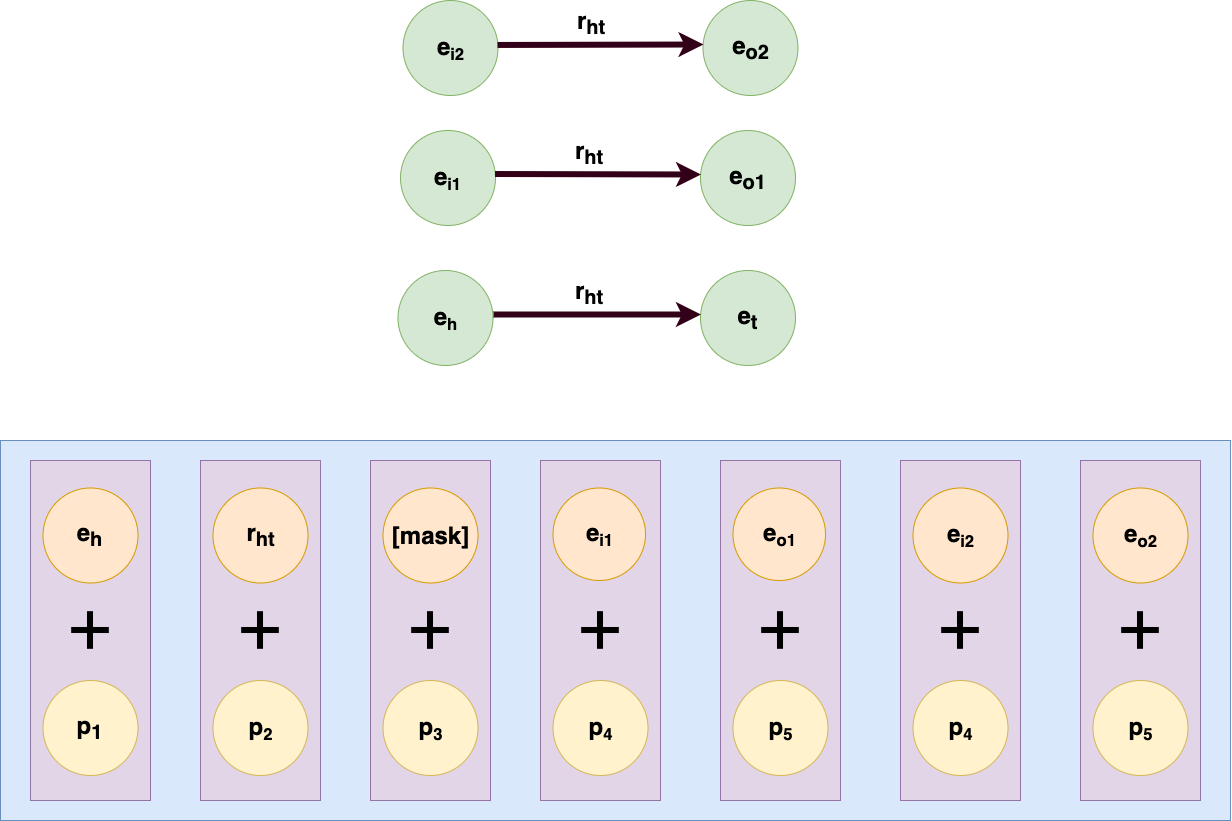
\includegraphics[scale=0.27]{similarity_based_model_output_variant}
\caption{An illustration of how similar entities are used to produce a training sample with a missing tail
entity.\ The top part of the figure illustrates a partially masked edge $(e_h, r_{ht}, e_t)$ along with sampled edges,
such that $e_{i1}$, $e_{i2}$ entities are similar to $e_h$.\ The bottom part shows how these edges are encoded into
input sequence pushed to the model.}
\label{fig:similarity_based_model_output_variant}
\end{figure}

\section{Training strategies}\label{sec:training_strategies}

There is nothing to prevent our models from being trained with multiple types of inputs, in particular those
discussed in \textit{Section} \ref{sec:context_models}.\ In our experiments, we test 3 different training strategies
to utilise various context types.\ Importantly, we keep positional embeddings of given triple's tokens fixed for all
input sequences, regardless of the specific context that is used.\ In contrast, tokens corresponding to different
contexts have disjoint positional embeddings.\ This allows the model to recognize different contexts, while
being aware of which tokens correspond to a considered triple.\newline

\noindent The first training strategy is to pretrain the model using different context types.\ More specifically,
given a probability distribution defining the probabilities of drawing specific context types, at each training step
one context type is sampled.\ Then, it is utilised to draw a batch of samples coming from the corresponding context's
dataset.\ The whole pretraining process can be thought of interleaving input sequences containing various
contexts.\ The probability distribution of selecting specific contexts is finetuned during the hyperparameter
optimization process.\ After the pretraining procedure, the model is trained without context to tune its parameters
to the final task of predicting a missing head/tail entity.\ The inference of the model on the the validation and test
datasets is performed on raw triples, without any context included.\ Therefore, other tasks are used only to train
better representations of entities and relations.\ We call this strategy of training the
\textbf{context-sampling strategy}.\newline

\noindent The other training strategy is to train the model with only one context type.\ In this setting, the model
is not trained on raw triples at all.\ Importantly, the inference on validation and test datasets is also performed by
constructing samples with a given context type.\ Intuitively, leveraging context information during the inference
can positively impact the performance on unseen examples.\ In case the context information is sampled, we find it
beneficial for our models to use the same context while doing the inference as during the training
process.\ We call the above-discussed strategy of training the \textbf{context-only strategy}.\newline

\noindent The last developed strategy of training is split into 2 phases.\ In the first phase, a separate transformer
model is trained for each context.\ This is motivated by the fact that when multiple contexts are used at the same
time, the model can learn to ignore some of them, particularly those that make up worse predictors.\ On the other
hand, sharing parameters of transformer layers between input sequences coming from different context types, can
encourage the model to memorize some parts of sequences.\ After each transformer model is trained, the training enters
into the second phase, in which another transformer is put on top the predicted embeddings.\ This allows the
embeddings to exchange information and as a result improve their representations.\ After that, each embedding is used
separately to compute a vector of similarities and the corresponding loss.\ Finally, all losses are summed up,
forming the total loss.\ We call the presented training strategy the \textbf{separate-contexts strategy}.

\section{Selected models}\label{sec:selected_models}

TODO

\numberedchapter{Experiments}\label{chapter:experiments}

As part of this thesis, we conducted several experiments applying our ideas presented in
\textit{Chapter} \ref{chapter:developed_methods}.\ Additionally, we compared the developed methods with competitive
baseline models presented in \textit{Section} \ref{sec:background_models}.\ The first sections of this chapter describe
the conducted experiments, while in the last section we present the obtained results.

\section{Datasets}

In the past, FB15K and WN18 datasets were used to evaluate the quality of knowledge graph completion models.\ After
it was noticed that a large number of test triplets can be obtained by inverting training triplets, the
\textbf{FB15K-237} and \textbf{WN18RR} datasets have been developed, reducing the above-mentioned problem.\ At this
time, knowledge graph completion models are mainly evaluated on these two datasets.\ Therefore, we evaluate our models
on FB15K-237 and WN18RR datasets.\newline

\noindent The FB15K-237 dataset is a subset of a large open-source knowledge base, called Freebase.\ It contains
relations between known people, movies, books, places and many others.\ The WN18RR dataset is a subset of WordNet,
forming a large database of English words.\ Its graph contains lexical and semantic relations.\ While the FB15K-237
dataset contains several hundreds relations, the WN18RR dataset contains only 11.\ Additionally, the former
one is much denser comparing the latter one.\ Therefore, the characteristics of both datasets are significantly
different.\ The precise statistics of both datasets are presented in \textit{Table} \ref{tab:datasets}.

\section{Metrics} \label{sec:metrics}

\noindent In order to evaluate a model on a set of triples $D$, we utilise several ranking-based
metrics for missing head and tail entities.\ Importantly, we do not use any triple contained in $D$ during the
evaluation of $d \in D$ i.e.\ the knowledge contained in other triples tested cannot be used to boost the predictions
for a specific $d \in D$.\ The metrics are calculated for each triple contained in $D$ and then averaged.\ Formally,
let $(h, r, t) = \tilde{d} \in D$ denote a triple to be evaluated.\ To prepare a ranking for a missing head of
$\tilde{d}$, we push a triple $([mask], r, t) = \tilde{d}_h \in D_h$ to a model.\ In case larger context is used by
the model, it is pushed along with $\tilde{d}_h$.\ The context includes only triples contained in the training
dataset, particularly triples from the validation dataset are not used when evaluating the quality of the test
dataset.\ As a result of this procedure, for each $\tilde{h} \in E$ we obtain a probability that
$(\tilde{h}, r, t) \in G$.\ The obtained vector of probabilities forms a ranking, where $\tilde{h}_1$ takes a higher
place than $\tilde{h}_2$ if and only if $P((\tilde{h}_1, r, t) \in G) > P((\tilde{h}_2, r, t) \in G)$.\ In case two
triples have been assigned the same probability, they are put on the same place in the ranking.\ The discussed procedure
forms an \textit{initial ranking} $R_{\tilde{d}, h}$ for $\tilde{d}_h$.\ The same procedure is repeated for
the tail entity $\tilde{d}_t$, forming an \textit{initial ranking} $R_{\tilde{d}, t}$.\newline

\noindent The \textit{initial ranking} is postprocessed in order to obtain the \textit{final ranking}.\ The first
step involves removing triples that are contained in either training, validation or test
dataset.\ This is known as a \textit{filtered} setting, firstly proposed in \cite{transe_model} and widely adopted in
other papers.\ Additionally, in case some probabilities outputted by the model correspond to other tokens than entities
(e.g.\ relations), they are removed from the ranking.\ Finally, draws are resolved by putting $(\tilde{h}_1, r, t)$
higher in the ranking than $(\tilde{h}_2, r, t)$ if and only if $\sigma(\tilde{h}_1) < \sigma(\tilde{h}_2)$, where
$\sigma$ denotes a predefined order-determining function.\ Importantly, $\sigma$ is fixed during the evaluation process
and corresponds to the order of entities in the vocabulary.\ We determined that the same order is used when the baseline
models have been evaluated by other authors.\ Performing the discussed steps on the given \textit{initial ranking}
$R_{\tilde{d}, h}$ (analogically $R_{\tilde{d}, t}$), forms the \textit{final ranking}
$\tilde{R}_{\tilde{d}, h}$ (analogically $\tilde{R}_{\tilde{d}, t}$) used to construct evaluation metrics.\newline

\begin{table}[!t]
\centering
\def\arraystretch{1.1}
\begin{tabular}{| l | r | r |}
 \hline
 \textbf{Statistic} & \textbf{FB15K-237} & \textbf{WN18RR} \\ [0.5ex]
 \Xhline{4\arrayrulewidth}
 \textbf{Entities} & 14,541 & 40,943 \\
 \hline
 \textbf{Relations} & 237 & 11 \\
 \hline
 \textbf{Training triples} & 272,115 & 86,835 \\
 \hline
 \textbf{Validation triples} & 17,535 & 3,034 \\
 \hline
 \textbf{Test triples} & 20,466 & 3,134 \\
 \hline
\end{tabular}
\caption{Statistics of FB15K-237 and WN18RR datasets.}
\label{tab:datasets}
\end{table}

\noindent Let us denote the position of the considered $\tilde{d}_h$ in the final ranking
$\tilde{R}_{\tilde{d}, h}$ (analogically $\tilde{R}_{\tilde{d}, t}$) as $r(\tilde{d}_h)$
(analogically $r(\tilde{d}_t)$).\ The \textbf{Mean Rank (MR)} metric is defined by the formula
$$
MR_h = \frac{1}{|D|} \sum_{\tilde{d}_h \in D} r(\tilde{d}_h)\ ,
$$
which is simply a mean of rankings.\ Similarly, the \textbf{Mean Reciprocal Rank (MRR)} metric is defined by
$$
MRR_h = \frac{1}{|D|} \sum_{\tilde{d}_h \in D} \frac{1}{r(\tilde{d}_h)}\ .
$$
In contrast to the MR metric, the higher MRR metric denotes the better score.\ Additionally, the score given by the
MRR metric grows exponentially with respect to the position in the ranking.\ As a result, improving the scores of
triples that are already high in the ranking is promoted more, compared to improving the scores of triples that are
low in the ranking.\ Lastly, the \textbf{Hits@10} metric is defined by the formula
$$
Hits@10_h = \frac{1}{|D|} \sum_{\tilde{d}_h \in D} \mathbbm{1}_{r(\tilde{d}_h) \leq 10}\ ,
$$
where $\mathbbm{1}_C$ is an indicator function that assigns $1$ if and only if a condition $C$ is satisfied and
otherwise it assigns $0$.\ Intuitively, the Hits@10 metric is the fraction of triples that were top 10 in the their
rankings.\newline

\noindent The above-defined metrics are calculated analogically for missing tail entities $D_t$, forming $MR_t$, $MRR_t$
and $Hits@10_t$ metrics.\ Finally, the same metrics are calculated for all samples $D_a = D_h \cup D_t$, forming $MR_a$,
$MRR_a$ and $Hits@10_a$ metrics.\ While we use head-specific and tail-specific metrics to debug our models, we report
only metrics for all samples, which we refer as $MR = MR_a$, $MRR = MRR_a$ and $Hits@10 = Hits@10_a$.\newline

\noindent As we mentioned above, draws are resolved by the order-determining function $\sigma$.\ While this is a
standard method at this time, in the recent past several researchers used another approach, causing the target triple
to be often higher in the ranking.\ More specifically, as it was shown in \cite{re_evaluation}, draws were resolved
by putting the target triple first in case it draws with other entities.\ As a result, models putting the same
probability for many entities performed very well, though their real quality was very poor.\ In particular, a model
assigning the same probabilities to all entities achieves the perfect score in this setting.\ In our experiments, we often
experienced this issue.\ Therefore, we decided to use order-determining function $\sigma$ and compare our methods only
with the models that have been evaluated or reevaluated using the same approach.

\section{Methodology}

Our models are trained on predefined training datasets of WN18RR and FB15K-237 knowledge bases.\ The predefined
validation datasets are used to estimate the quality of models every few thousand steps.\ The total number of training
steps depend on whether validation metrics indicate some progress.\ Specifically, in case the MRR metric on validation
dataset is lower than the best one, 5 times in a row, the training procedure is stopped.\ The maximum
number of possible training steps is set to 160,000, which corresponds to a few hundred epochs for both datasets.\ In
practice, most of trained models converge after about 40,000 steps.\ After the training procedure, the model's state
corresponding to the highest MRR value is chosen and saved.\newline

\noindent We run the training procedure several times, each time sampling hyperparameters
from the predefined set.\ In particular, for all models we finetune the initial learning rate along
with decay rate, dropout rate, weight decay, label smoothing, activation function used in all layers, the dimensions
of embeddings and layers, the number of attention heads in each layer and a standard deviation $\sigma$ of initial
parameters (truncated normal distribution is used for initialization).\ While the optimal values for most of
the above-mentioned parameters are model-specific, we found that poor initialization leads the models to be stuck,
making no progress.\ Therefore, learnable parameters of all models are initialized with
$\sigma \in [0.01, 0.03]$.\ Additionally, we noticed that setting label smoothing $s$ to a high value
$s \in [0.7, 0.85]$ consistently provides better results.\ We also noticed a positive impact of applying dropout layers
and weight decay.\ For all models, the optimal number of embeddings dimensions $d_e$ was in $d_e \in [256, 512]$ range,
while the optimal number of attention heads $n_a$ lied in $n_a \in [4, 8]$ range.\ Furthermore, the optimal number of
dimensions of attention heads and pointwise feed-forward layers lied in $[256, 512]$ and $[512, 1024]$ ranges,
respectively.\ Lastly, we found that the best models use learning rate $\alpha$ in range $\alpha \in [0.0001, 0.0005]$
and linear decay with rate $0.0625$ i.e.\ the learning rate of the last step is equal to $0.0625\times \alpha$ and the
learning rate of intermediate steps scales linearly.\newline

\noindent The process of finding the best hyperparameters is repeated for each of the proposed models, forming separate
categories.\ Afterwards, the best model for each category is chosen based on the MRR metric.\ In order to assess the
quality of the chosen models, each of them is evaluated on the predefined test dataset.\ Additionally, we reproduce
TransE, STransE and ConvE models, achieving similar results to those presented in other papers.\ Nevertheless, we
compare our models with the results presented in original papers.\ In case, an original paper does not use the same
evaluation protocol as the one discussed in \textit{Section} \ref{sec:metrics}, we rely on reevaluations performed by
other researchers.

\section{The obtained results}

\noindent Lorem ipsum dolor sit amet, consectetur adipiscing elit, sed do eiusmod tempor incididunt ut
labore et dolore magna aliqua. Ut enim ad minim veniam, quis nostrud exercitation ullamco laboris nisi
ut aliquip ex ea commodo consequat. Duis aute irure dolor in reprehenderit in voluptate velit esse
cillum dolore eu fugiat nulla pariatur. \newline

\noindent Lorem ipsum dolor sit amet, consectetur adipiscing elit, sed do eiusmod tempor incididunt ut
labore et dolore magna aliqua. Ut enim ad minim veniam, quis nostrud exercitation ullamco laboris nisi
ut aliquip ex ea commodo consequat. Duis aute irure dolor in reprehenderit in voluptate velit esse
cillum dolore eu fugiat nulla pariatur. \newline

\begin{table}[!t]
\centering
\def\arraystretch{1.1}
\begin{tabular}{|l || r | r | r || r | r | r |}
 \hline
 \multirow{2}{*}{\textbf{Model}} & \multicolumn{3}{c||}{\textbf{FB15K-237}} & \multicolumn{3}{c|}{\textbf{WN18RR}} \\
 \cline{2-7}
 & \textbf{MRR} $\uparrow$ & \textbf{MR} $\downarrow$ & \textbf{Hits@10} $\uparrow$ & \textbf{MRR} $\uparrow$ &
 \textbf{MR} $\downarrow$ & \textbf{Hits@10} $\uparrow$ \\
 \Xhline{4\arrayrulewidth}
 \textbf{TransE} & 0.294 & 357 & 0.465 & 0.226 & 3384 & 0.501 \\
 \hline
 \textbf{STransE} & 0.312 & - & 0.480 & 0.251 & - & 0.509 \\
 \hline
 \textbf{ConvE} & 0.325 & 244 & 0.501 & 0.430 & 4187 & 0.520 \\
 \hline
 \textbf{MINERVA} & 0.293 & - & 0.513 & 0.448 & - & 0.456 \\
 \hline
 \textbf{SACN} & 0.350 & - & 0.540 & 0.470 & - & 0.540 \\
 \hline
 \textbf{CompGCN} & 0.355 & 197 & 0.535 & 0.479 & 3533 & 0.546 \\
 \hline
 \textbf{Ours1} & ? & ? & ? & ? & ? & ? \\
 \hline
 \textbf{Ours2} & ? & ? & ? & ? & ? & ? \\
 \hline
 \textbf{Ours3} & ? & ? & ? & ? & ? & ? \\
 \hline
 \textbf{Ours4} & ? & ? & ? & ? & ? & ? \\
 \hline
 \textbf{Ours5} & ? & ? & ? & ? & ? & ? \\
 \hline
\end{tabular}
\caption{Knowledge graph completion results on FB15K-237 and WN18RR test datasets.\ Note that some authors have not
evaluated their models on MR metric.}
\label{tab:full_results}
\end{table}

\noindent Lorem ipsum dolor sit amet, consectetur adipiscing elit, sed do eiusmod tempor incididunt ut
labore et dolore magna aliqua. Ut enim ad minim veniam, quis nostrud exercitation ullamco laboris nisi
ut aliquip ex ea commodo consequat. Duis aute irure dolor in reprehenderit in voluptate velit esse
cillum dolore eu fugiat nulla pariatur. \newline


\numberedchapter{Summary}

In this thesis, we explored how transformed-based models can be applied to the knowledge graph completion
problem.\ To reach our first milestone of outperforming context-free baseline methods, we developed an architecture
operating on triples alone.\ We showed that it is superior to other methods in this category and presented the
importance of the developed components, performing an extensive hyperparameters fine-tuning.\ In the next part of this
thesis, we extended our model to include the context extracted from the graph representation of training data.\ We
presented various approaches to apply this idea and conducted several experiments measuring the impact of each
modification.\ Furthermore, we compared our models with context-free, reinforcement learning and graph neural networks
approaches.\ The developed methods were superior to context-free and reinforcement learning models, while the
best-performing graph neural network model achieved similar quality.\ We can conclude that transformer-based methods
are competitive with the current state of the art methods, even when no context information is used or it is much
smaller compared to other methods, which aggregate information from multi-hop neighbourhood.

\section{Future work}

Although transformers proved to provide a significant improvement over other methods, adding the context to the model
boost the performance only slightly.\ In other words, the transformer architecture operating on triples alone provide
a surprisingly high quality boost, while context-based transformer models only add a little bit of extra quality.\ The
same pattern can be observed when applying graph convolutional networks on top of other methods.\ It is an open
question whether it means that the context information is not so useful in the knowledge graph completion problem
or the explored methods fail to extract it.\ One of the unexplored direction of future research is to combine
transformer-based and graph-based methods.\ For instance, the CompGCN model could be used to aggregate information from
the distant neighbourhood, while the transformer model could be applied on the aggregated embeddings.\ The other idea
would be to stack a few transformers, one on top of each other.\ While this may sound like a graph neural network model,
the transformers can be stacked in more custom ways, allowing layer-specific aggregations.\ Additionally, several
extensions to the transformer architecture keep coming up and could be tried out to tackle the considered
problem.\ One of recently developed pre-training methods include ELECTRA, discussed in
\textit{Subsection} \ref{subsec:transformer_extensions}.\ This method could be used to pretrain our model on long paths
with some entities masked out.

\section{Acknowledgments}

I would like to thank my supervisor dr hab.\ Jan Chorowski from the Institute of Computer Science at the
University of Wrocław for his assistance on this project and bringing in new ideas.\ I really appreciate his time
devoted to me during the development of this thesis.

\begin{thebibliography}{99}

\bibitem{transe_model}
Antoine Bordes, Nicolas Usunier, Alberto Garcia-Duran, Jason Weston, Oksana Yakhnenko - \textit{Translating Embeddings
for Modeling Multi-relational Data (2013)}

\bibitem{skipgram}
Tomas Mikolov, Ilya Sutskever, Kai Chen, Greg Corrado, Jeffrey Dean - \textit{Distributed Representations of
Words and Phrases and their Compositionality (2013)}

\bibitem{gan}
Ian J. Goodfellow, Jean Pouget-Abadie, Mehdi Mirza, Bing Xu, David Warde-Farley, Sherjil Ozair, Aaron Courville,
Yoshua Bengio - \textit{Generative Adversarial Nets (2014)}

\bibitem{dropout}
Nitish Srivastava, Geoffrey Hinton, Alex Krizhevsky, Ilya Sutskever, Ruslan Salakhutdinov - \textit{Dropout: A
Simple Way to Prevent Neural Networks from Overfitting (2014)}

\bibitem{deepwalk}
Bryan Perozzi, Rami Al-Rfou, Steven Skiena - \textit{DeepWalk: Online Learning of Social Representations (2014)}

\bibitem{batch_normalization}
Sergey Ioffe, Christian Szegedy - \textit{Batch Normalization: Accelerating Deep Network Training by
Reducing Internal Covariate Shift (2015)}

\bibitem{adam_optimizer}
Diederik P. Kingma, Jimmy Lei Ba - \textit{Adam: A method for stochastic optimization (2015)}

\bibitem{reinforcement_learning_book}
Richard S. Sutton and Andrew G. Barto - \textit{Reinforcement Learning: An Introduction (2015)}

\bibitem{layer_normalization}
Jimmy Lei Ba, Jamie Ryan Kiros, Geoffrey E. Hinton - \textit{Layer Normalization (2015)}

\bibitem{goodfellow_book}
Ian Goodfellow, Yoshua Bengio, Aaron Courville - \textit{Deep learning (2016)}

\bibitem{node2vec}
Aditya Grover, Jure Leskovec - \textit{node2vec: Scalable Feature Learning for Networks (2016)}

\bibitem{planetoid}
Zhilin Yang, William W. Cohen, Ruslan Salakhutdinov - \textit{
Revisiting Semi-Supervised Learning with Graph Embeddings (2016)}

\bibitem{sdne}
Daixin Wang, Peng Cui, Wenwu Zhu - \textit{Structural Deep Network Embedding (2016)}

\bibitem{struc2vec}
Leonardo F. R. Ribeiro, Pedro H. P. Saverese, Daniel R. Figueiredo - \textit{struc2vec: Learning Node
Representations from Structural Identity (2017)}

\bibitem{stranse_model}
Dat Quoc Nguyen, Kairit Sirts, Lizhen Qu, Mark Johnson - \textit{STransE: a novel embedding model of entities and
relationships in knowledge bases (2017)}

\bibitem{graphsage}
William L. Hamilton, Rex Ying, Jure Leskovec - \textit{Inductive Representation Learning on Large Graphs (2017)}

\bibitem{transformer_model}
Ashish Vaswani, Noam Shazeer, Niki Parmar, Jakob Uszkoreit, Llion Jones, Aidan N. Gomez, Łukasz Kaiser,
Illia Polosukhin - \textit{Attention Is All You Need (2017)}

\bibitem{convkb_model}
Dai Quoc Nguyen, Tu Dinh Nguyen, Dat Quoc Nguyen, Dinh Phung - \textit{A Novel Embedding Model for Knowledge Base
Completion Based on Convolutional Neural Network (2018)}

\bibitem{conve_model}
Tim Dettmers, Pasquale Minervini, Pontus Stenetorp, Sebastian Riedel - \textit{Convolutional 2D Knowledge
Graph Embeddings (2018)}

\bibitem{gat}
Petar Velickovic, Guillem Cucurull, Arantxa Casanova, Adriana Romero, Pietro Lio, Yoshua Bengio - \textit{Graph
attention networks (2018)}

\bibitem{go_for_a_walk_model}
Rajarshi Das, Shehzaad Dhuliawala, Manzil Zaheer, Luke Vilnis, Ishan Durugkar, Akshay Krishnamurthy, Alex Smola,
Andrew McCallum - \textit{Go for a walk and arrive at the answer: reasoning over paths in knowledge bases using
reinforcement learning (2018)}

\bibitem{sacn_model}
Chao Shang, Yun Tang, Jing Huang, Jinbo Bi, Xiaodong He, Bowen Zhou - \textit{
End-to-end Structure-Aware Convolutional Networks for Knowledge Base Completion (2018)}

\bibitem{gcn_model}
Chao Shang, Yun Tang, Jing Huang, Jinbo Bi, Xiaodong He, Bowen Zhou - \textit{End-to-end Structure-Aware
Convolutional Networks for Knowledge Base Completion (2018)}

\bibitem{bert_model}
Jacob Devlin, Ming-Wei Chang, Kenton Lee, Kristina Toutanova - \textit{BERT: Pre-training of Deep Bidirectional
Transformers for Language Understanding (2019)}

\bibitem{layer_normalization_in_transformers}
Ruibin Xiong, Yunchang Yang,  Di He, Kai Zheng, Shuxin Zheng, Chen Xing, Huishuai Zhang, Yanyan Lan,
Liwei Wang, Tie-Yan Liu - \textit{On Layer Normalization in the Transformer Architecture (2020)}

\bibitem{albert_model}
Zhenzhong Lan, Mingda Chen, Sebastian Goodman, Kevin Gimpel, Piyush Sharma, Radu Soricut - \textit{ALBERT: a
lite BERT for self-supervised learning of language representations (2020)}

\bibitem{electra_model}
Kevin Clark, Minh-Thang Luong, Quoc V. Le, Christopher D. Manning - \textit{Electra: pre-training text encoders
as discriminators rather than generators (2020)}

\bibitem{re_evaluation}
Farahnaz Akrami, Lingbing Guo, Wei Hu, Chengkai Li - \textit{Re-evaluating Embedding-Based Knowledge Graph
Completion Methods (2020)}

\bibitem{comp_gcn_model}
Shikhar Vashishth, Soumya Sanyal, Vikram Nitin, Partha Talukdar - \textit{Composition-based multi-relational graph
convolutional networks (2020)}

\end{thebibliography}
\addcontentsline{toc}{chapter}{Bibliography}

\end{document}
